\documentclass[11pt]{article}
\usepackage[a4paper,margin=18mm]{geometry}
\usepackage[no-math]{fontspec}
\setmainfont{Latin Modern Roman}
\usepackage{amsmath,amssymb,amsthm,xfrac,xspace,hyperref,graphicx,comment}
\excludecomment{DefTralics}

\providecommand{\bibliofont}{\small}
\newcommand{\ie}{i.e.,\xspace}
\newcommand{\eg}{e.g.,\xspace}
\newcommand{\etc}{etc.\xspace}
\newcommand{\cf}{cf.\xspace}
\newcommand{\resp}{resp.\xspace}
\newcommand{\smaller}{\small}
\newcommand{\Subsection}{\subsection}
\newcommand{\Subsubsection}{\subsubsection}
\newcommand{\skpt}{\smallskip}
\emergencystretch=3em
\numberwithin{equation}{section}
% Begin literal retained input author-preamble.tex
\usepackage{mathrsfs}
% Retained existing local compatibility package bbm


\let\mathcal\mathscr
\usepackage{tikz}
\usetikzlibrary{cd}
\tikzcdset{arrow style=Latin Modern}
\newcommand{\dradpl}{{\hspace*{-2.5mm}\begin{tikzcd}[ampersand replacement=\&,column sep = scriptsize]\mbox{}\ar[r,dashed]\&\mbox{}\end{tikzcd}\hspace*{-2.5mm}}}
\newcommand{\dratst}{{\hspace*{-2.5mm}\begin{tikzcd}[ampersand replacement=\&,column sep = small]\mbox{}\ar[r,dashed]\&\mbox{}\end{tikzcd}\hspace*{-2mm}}}
\let\drascst\dratst
\newcommand{\dra}{\mathchoice{\dradpl}{\dratst}{\drascst}{\drascst}}

\def\mto{\mathchoice{\longmapsto}{\mapsto}{\mapsto}{\mapsto}}
\def\hto{\mathrel{\lhook\joinrel\to}}

\renewcommand{\labelitemi}{$\scriptstyle\bullet$}
\newcommand{\ra}{\mathrm{a}}
\let\oldvee\vee
\renewcommand{\vee}{{\scriptscriptstyle\oldvee}}
\let\oldbot\bot
\renewcommand{\bot}{{\scriptscriptstyle\oldbot}}

\usepackage[all,cmtip]{xy}\let\labelstyle\textstyle

% Retained existing local compatibility package stmaryrd
\RequirePackage{fontspec}
\newfontfamily\jepTagFont[ItalicFont={Noto Sans Math},BoldFont={Noto Sans Math},BoldItalicFont={Noto Sans Math}]{Noto Sans Math}
\newcommand{\varocircle}{\bigcirc}
\newcommand{\varominus}{\mathord{\text{\jepTagFont\upshape\char"2296}}}
\newcommand{\varobar}{\mathord{\text{\jepTagFont\upshape\char"29B6}}}
\newcommand{\boxbox}{\mathord{\text{\jepTagFont\upshape\char"29C8}}}


\usepackage{mathtools}
\usepackage{pgfplots}
\pgfplotsset{compat=1.17}
\usepackage{xcolor}

\colorlet{lightlightgray}{gray!20}
\colorlet{light1.5gray}{gray!35}

\theoremstyle{plain}
\newtheorem{theorem}{Theorem}[section]
\newtheorem{lemma}[theorem]{Lemma}
\newtheorem{corollary}[theorem]{Corollary}
\newtheorem{proposition}[theorem]{Proposition}
\newtheorem{question}[theorem]{Question}
\newtheorem{maintheorem}{Main Theorem}
\renewcommand\themaintheorem{\Alph{maintheorem}}
\newtheorem{introtheorem}{Theorem}

\theoremstyle{definition}
\newtheorem{introremark}[introtheorem]{Remark}
\newtheorem{remark}[theorem]{Remark}
\newtheorem{example}[theorem]{Example}
\newtheorem{definition}[theorem]{Definition}

\DeclareMathOperator{\SL}{SL}
\DeclareMathOperator{\Lie}{Lie}
\DeclareMathOperator{\pr}{pr}
\DeclareMathOperator{\Aut}{Aut}
\DeclareMathOperator{\Spec}{Spec}
\DeclareMathOperator{\Hom}{Hom}
\DeclareMathOperator{\rank}{rank}
\DeclareMathOperator{\aff}{aff}
\DeclareMathOperator{\Ve}{Vec}
\DeclareMathOperator{\LND}{LND}
\DeclareMathOperator{\Conv}{Conv}
\DeclareMathOperator{\Span}{Span}
\DeclareMathOperator{\Mor}{Mor}
\DeclareMathOperator{\Der}{Der}
\DeclareMathOperator{\inter}{int}

\newcommand{\norm}[1]{\left\lVert#1\right\rVert}
\newcommand{\OO}{\mathcal{O}}
\newcommand{\GG}{\mathbb{G}}
\newcommand{\RR}{\mathbb{R}}
\newcommand{\ZZ}{\mathbb{Z}}
\renewcommand{\AA}{\mathbb{A}}

\newcommand{\kk}{{\boldsymbol{k}}}

\newcommand{\aquot}{/ \! \! /}

\newcommand{\name}[1]{#1}

\let\phi\varphi

\newcommand{\set}[2]{\{#1 \mid #2\}}
\newcommand{\bset}[2]{\bigl\{#1 \mid #2\bigr\}}
\newcommand{\Bigset}[2]{\biggl\{#1 \Bigm|  #2\biggr\}}
\newcommand{\sprod}[2]{\langle #1, #2 \rangle}


% End literal retained input author-preamble.tex

\makeatletter
\renewcommand\section{\@startsection{section}{1}{\z@}{-3.5ex \@plus -1ex \@minus -.2ex}{2.3ex \@plus .2ex}{\normalfont\large\bfseries}}
\makeatother
\begin{document}
\begin{center}{\Large Stable item 2046}\end{center}
\paragraph{Source and attribution.}
Andriy Regeta, Immanuel van Santen, \emph{Characterizing smooth affine spherical varieties via the automorphism group}, Journal de l’École polytechnique — Mathématiques 8 (2021), publisher version, DOI 10.5802/jep.149. \href{https://jep.centre-mersenne.org/articles/10.5802/jep.149/}{Publisher article}. Authors' text: \href{https://creativecommons.org/licenses/by/4.0/}{CC BY 4.0}.
\paragraph{Editorial problem boundary.}
Prove only Proposition 7.3 below over an algebraically closed characteristic-zero field, for an irreducible quasi-affine variety with faithful action of a connected solvable group containing nontrivial unipotent elements. The open-orbit condition is equivalent to the printed bounded semi-invariant vector-field spaces and bounded generalised root subgroups. The complete equal-weight semi-invariant and arbitrarily large faithful replicated additive-action construction is retained. Reductive reconstruction, arbitrary torus actions and later weight-monoid formulae are context only.
\paragraph{Difficulty (editorial): H2.}
The cited rational quotient and solvable invariant-fraction results do not by themselves produce root subgroups of a prescribed common weight and arbitrarily large dimension. The author combines two equal-weight semi-invariants with a homogeneous additive action to construct the displayed replicated actions, and verifies faithfulness through the independence of their homogeneous powers. That same-weight replication construction supplies the unbounded family needed for the converse implication, together with the exact vector-field/root-subgroup comparison.
\paragraph{Editorial transcription note.}
Original author language, mathematics and ordering are preserved. Publisher front matter is replaced by this independent article wrapper. Bibliography is recovered from matching cached publisher HTML, including its TeX formulas. No new proof or mathematical repair is supplied. Surrounding original results are retained for conservative context and are not extra selected corpus claims.
\clearpage

% Begin literal retained input author-body.tex
\section{Introduction}

In this article, we work over an algebraically closed field $\kk$ of characteristic zero
if it is not specified
otherwise.

In \cite[Th.\,1.1]{Kraft2017}, \name{Kraft} proved
that $\mathbb{A}^n$ is determined by
its automorphism group $\Aut(\AA^n)$ seen as an ind-group
inside the category of connected affine varieties
(see~\cite{FuKr2018On-the-geometry-of} for a reference of ind-groups) and in \cite[Main Th.]{KrReSa2018Is-the-affine-spac},
this result was partially generalized (over the complex numbers)
in case $\Aut(\AA^n)$ is seen only as an abstract group.
In \cite[Th.\,A]{CaReXi2019Families-of-Commut},
the last results are widely generalized in the following sense:
$\AA^n$ is completely characterized through the abstract group
$\Aut(\AA^n)$ inside the category of connected affine varieties.
The result of \name{Kraft} was partially generalized (over the complex numbers) to other affine varieties
than the affine space in \cite{Re2017Characterization-o} and \cite{LiReUr2018Characterization-o}.
More precisely, there is the following statement
(formulated over the complex numbers, but valid with the same proof over $\kk$):

\begin{introtheorem}[{\cite[Th.\,1.4]{LiReUr2018Characterization-o}}]
\label{theorem0}
Let $X$ be an affine toric variety different from the torus
and let $Y$ be an irreducible normal affine variety. If $\Aut(X)$ and $\Aut(Y)$ are isomorphic
as ind-groups, then $X$ and $Y$ are isomorphic as varieties.
\end{introtheorem}

\begin{introremark}
\label{rem.Theorem0}
In fact, in both \cite{Kraft2017} and \cite[Th.\,1.4]{LiReUr2018Characterization-o}, the
authors prove the statements under the slightly weaker assumption
that there is a group isomorphism $\Aut(X) \simeq \Aut(Y)$
that preserves algebraic subgroups (see Section~\ref{sec.AutomorphismGroups} for the definition).
\end{introremark}

A natural generalization of toric varieties are the so-called spherical varieties.
Let~$G$ be a connected reductive algebraic group.
Recall that a normal variety $X$ endowed with a faithful $G$-action
is called \emph{$G$-spherical} if some (and hence every)
Borel subgroup in $G$ acts on $X$ with an open dense orbit, see
\eg \cite{Br2010Introduction-to-ac} for a survey
and~\cite{Ti2011Homogeneous-spaces} for a reference of the topic. If $G$ is a torus, then a $G$-spherical variety is the same thing as a $G$-toric variety.
If $X$ is $G$-spherical, then
$X$ has an open $G$-orbit which is isomorphic to $G/H$ for some subgroup $H \subset G$.
The family of $G$-spherical varieties is, in~a sense, the widest family of $G$-varieties which is well-studied: in fact, $G$-equivariant open embeddings of $G$-homogeneous
$G$-spherical varieties are classified
by certain combinatorial data (analogous to the classical case of toric varieties)
by \name{Luna-Vust} \cite{LuVu1983Plongements-despac} (see also the work of \name{Knop} \cite{Kn1991The-Luna-Vust-theo})
and homogeneous $G$-spherical varieties are classified for $\kk$ equal to the complex numbers
by \name{Luna}, \name{Bravi}, \name{Cupit-Foutou}, \name{Losev} and \name{Pezzini}
\cite{Lu2001Varietes-spherique, BrPe2005Wonderful-varietie, Br2007Wonderful-varietie,
Lu2007La-variete-magnifi, Lo2009Uniqueness-propert, BrCu2010Classification-of-, Cu2014Wonderful-Varietie}.

In this paper, we generalize partially Theorem \ref{theorem0} to quasi-affine $G$-spherical varieties.
In order to state our main results, let us introduce some notation. Let
$X$ be an irreducible $G$-variety for a connected algebraic group $G$ with a fixed Borel subgroup
$B \subset G$.
We denote by $\mathfrak{X}(B)$ the character group
of $B$, \ie the group of regular group homomorphisms $B \to \GG_m$.
The \emph{weight monoid} of $X$ is defined by
\[
\Lambda^+(X) = \{\lambda \in \mathfrak{X}(B) \mid \OO(X)_{\lambda}^{(B)} \neq 0\},
\]
where $\OO(X)_{\lambda}^{(B)} \subset \OO(X)$
denotes the subspace of $B$-semi-invariants of weight $\lambda$
of the coordinate ring $\OO(X)$ of $X$, \ie
\[
\OO(X)_{\lambda}^{(B)} = \set{f \in \OO(X)}{b \cdot f = \lambda(b) f \ \textrm{for all $b \in B$}}.
\]
Our main result in this article is the following:

\begin{maintheorem}
\label{mainthm:autos}
Let $X$, $Y$ be irreducible normal quasi-affine varieties, let
$\theta \colon \Aut(X) \simeq \Aut(Y)$ be a group isomorphism
that preserves algebraic subgroups (see Section~\ref{sec.AutomorphismGroups} for the definition)
and let $G$ be a connected reductive
algebraic group.
Moreover, we fix a Borel subgroup $B \subset G$.
If $X$ is $G$-spherical and not isomorphic to a torus, then the following holds:
\begin{enumerate}
\item \label{main1} $Y$ is $G$-spherical for the induced $G$-action via $\theta$;
\item \label{main2} the weight monoids $\Lambda^+(X)$ and $\Lambda^+(Y)$ inside $\mathfrak{X}(B)$
are the same;
\item \label{main3} if one of the following assumptions holds
\begin{enumerate}\renewcommand{\theenumii}{\roman{enumii}}
\item \label{main3smooth} $X$, $Y$ are smooth and affine or
\item \label{main3toric} $X$, $Y$ are affine and $G$ is a torus,
\end{enumerate}
then $X$ and $Y$ are isomorphic as $G$-varieties.
\end{enumerate}
\end{maintheorem}

We prove Main Theorem~\ref{mainthm:autos}\eqref{main1} in Proposition~\ref{prop.iso_and_sphericity},
Main Theorem~\ref{mainthm:autos}\eqref{main2} in Corollary~\ref{thesameweights}
and Main Theorem~\ref{mainthm:autos}\eqref{main3} in Theorem~\ref{thm.smooth_spherical_var}.

In case $X$ is isomorphic to a torus and $X$ is $G$-spherical, it follows that $G$ is in fact a torus
of dimension $\dim X$. Indeed, as each unipotent closed subgroup of $G$ acts trivially on
$X \simeq (\kk^\ast)^{\dim X}$ and since $G$ acts faithfully on $X$, it follows that $G$ has no unipotent
elements; hence $G$ is a torus \cite[Prop.\,B, \S21.4]{Hu1975Linear-algebraic-g}. Thus $X\simeq G$.
Then \cite[Exam.\,6.17]{LiReUr2018Characterization-o} gives an example
of an affine variety $Y$ such that there is a group isomorphism $\theta \colon \Aut(X) \to \Aut(Y)$
that preserves algebraic subgroups, but~$Y$ is not $G$-toric. Thus the assumption that $X$ is
not isomorphic to a torus in Main Theorem~\ref{mainthm:autos} is essential.

Moreover, in general, we cannot drop the normality condition in Main Theorem~\ref{mainthm:autos}:
We provide an example in Proposition~\ref{prop.ex_normality} where the weight monoids of $X$ and $Y$ are different,
see Section~\ref{sec.Counter_example}.

\subsection*{Outline of the proof of Main Theorem~\ref{mainthm:autos}\eqref{main1}}
We introduce \emph{generalized root subgroups} of $\Aut(X)$ and study these subgroups and
their weights for a $G$-variety $X$ (see Section~\ref{sec.determination_of_sphericity} for details).
We show that if $G$ is not a torus,
then an irreducible normal quasi-affine variety with a faithful $G$-action is
$G$-spherical if and only if the dimension of all
generalized root subgroups of $\Aut(X)$ with respect to $B$
is bounded (see Definition~\ref{def.generalized_root_subgroup}, Proposition~\ref{prop:characterization_of_aff_spherical_var} and Lemma~\ref{lem.B_contains_unipotent_elements}). This characterization of the sphericity
is stable under
group isomorphisms of automorphism groups that preserve algebraic groups
and thus we get Main Theorem~\ref{mainthm:autos}\eqref{main1}.

\subsection*{Outline of the proof of Main Theorem~\ref{mainthm:autos}\eqref{main2}}
We show
that the weight monoid $\Lambda^+(X)$ of a quasi-affine
$G$-spherical variety $X$ is encoded in
the following set:
\[
D(X) = \Bigset{ \lambda \in \mathfrak{X}(B)}{
\begin{array}{l}
\textrm{there exists a non-trivial $B$-homogeneous} \\
\textrm{$\GG_\ra$-action on $X$ of weight $\lambda$}
\end{array}
}
\]
(see Section~\ref{sec.GroupActionsAndVectorfields} for the definition of a $B$-homogeneous $\GG_\ra$-action). We call $D(X)$ \emph{the set of $B$-homogeneous $\GG_\ra$-weights} of $X$.
To $D(X) \subset \mathfrak{X}(B)$ we may associate its asymp\-totic cone $D(X)_{\infty}$ inside
$\mathfrak{X}(B) \otimes_\ZZ \RR$ and consider the convex cone $\Conv ( D(X)_{\infty})$
of~it (see Section~\ref{sec.Cones_and_asymptotic_cones} for the definitions).
We prove then the following ``closed formula'' for the weight monoid:

\begin{maintheorem}
\label{mainthm:closed_formula}
Let $G$ be a connected reductive algebraic group, $B \subset G$ a Borel subgroup, and
$X$ a quasi-affine $G$-spherical variety that is non-isomorphic to a torus.
If neither $G$ is a torus nor $\Spec(\OO(X)) \not\simeq \AA^1 \times (\AA^1 \setminus \{0\})^{\dim(X)-1}$, then
\[
\Lambda^+(X) = \Conv ( D(X)_{\infty}) \cap \Span_{\ZZ}(D(X)),
\]
where the asymptotic cones and linear spans are taken inside $\mathfrak{X}(B) \otimes_{\ZZ} \RR$.
\end{maintheorem}

Main Theorem~\ref{mainthm:closed_formula} is proved in Theorem~\ref{thm.description_of_weight-monoid}.
As a consequence of this result, we get that the set of $B$-homogeneous $\GG_\ra$-weights
determines the weight monoid, see Corollary~\ref{cor.weights_describe_weight-monoid}:

\begin{maintheorem}
\label{main_weight_monoid}
Let $G$ be a connected reductive algebraic group and let
$X, Y$ be quasi-affine $G$-spherical varieties with $D(X) = D(Y)$. Then $\Lambda^+(X) = \Lambda^+(Y)$.
\end{maintheorem}

Using this last result, we get then Theorem~\ref{mainthm:autos}\eqref{main2},
as the existence of a group isomorphism $\Aut(X) \to \Aut(Y)$ that preserves algebraic groups
implies that $D(X) = D(Y)$, see Lemma~\ref{lem.auto_perserves_weights}.

\subsection*{Outline of the proof of Main Theorem~\ref{mainthm:autos}\eqref{main3}}
Note that the statement of Main Theorem~\ref{mainthm:autos}\eqref{main3toric} is
the same as Theorem~\ref{theorem0}
together with Remark~\ref{rem.Theorem0}. We mentioned it here as it is a
direct consequence of Main Theorem~\ref{mainthm:autos}\eqref{main2}.
Again using Main Theorem~\ref{mainthm:autos}\eqref{main2},
the statement of Main Theorem~\ref{mainthm:autos}\eqref{main3smooth} is a direct
consequence of the following beautiful result of \name{Losev}
that proves \name{Knop}'s Conjecture:

\begin{introtheorem}[{\cite[Th.\,1.3]{Lo2009Proof-of-the-Knop-}}]
\label{thm.losev}
If $X$ and $Y$ are smooth affine $G$-spherical varieties with $\Lambda^+(X) = \Lambda^+(Y)$,
then $X$ and $Y$ are isomorphic as $G$-varieties.
\end{introtheorem}

\subsection*{Outline of the structure of the paper }
In Section~\ref{sec.Cones_and_asymptotic_cones} we introduce the concept of the
asymptotic cone $D_{\infty}$ associated to a given set $D$ in a Euclidean vector space.
One can think of $D_{\infty}$ as the set one receives if one looks at $D$ from
``infinitely far away''. We provide in this Section several properties of (asymptotic) cones used
for our study of homogeneous $\GG_\ra$-actions on toric varieties in Section~\ref{sec.homogeneou_Ga-actions_quasi-affine} and also for the proof of
our ``closed formula'' of the weight monoid in terms of the set of homogeneous $\GG_\ra$-weights,
\ie Main Theorem~\ref{mainthm:closed_formula}.

In Sections~\ref{sec.Quasi-affine}, ~\ref{sec.vectorfields}, ~\ref{sec.AutomorphismGroups}
we gather general results about quasi-affine varieties,
vector fields, automorphism groups of varieties and root subgroups.
This material is constantly used in the rest of the article.
For several results we don't have an appropriate reference to the literature and
thus we provide full proofs.

In Section~\ref{sec.homogeneou_Ga-actions_quasi-affine} we study homogeneous $\GG_\ra$-actions
on quasi-affine toric varieties. Let~us highlight the two main results. For this, let
$X$ be a quasi-affine toric variety described by some fan $\Sigma$ of convex cones.
Then the associated affine variety $X_{\aff} \coloneqq \Spec(\OO(X))$
is again toric (see Lemma~\ref{lem:Spherical_quasi-affine}) and thus can
be described by some convex cone $\sigma$.
Our first main result in this section (Corollary~\ref{Cor:Classification_LND_Quasi-affine})
provides
a full description of the homogeneous $\GG_\ra$-actions on $X$ in terms of the fan $\Sigma$.
In our second main result (Corollary~\ref{cor.Weights})
we describe the asymptotic cone of the set $D(X)$
of homogeneous $\GG_\ra$-weights of $X$ in terms of the convex cone $\sigma$.

In Section~\ref{sec.determination_of_sphericity} we show that the automorphism
group determines the sphericity, \ie we prove~Main Theorem~\ref{mainthm:autos}\eqref{main1}.
As already mentioned, the idea is to characterize the sphericity in terms of so-called
generalized root subgroups, see Proposition~\ref{prop:characterization_of_aff_spherical_var}.

In Section~\ref{sec.relation_homogen_Ga-weights_weight_monoid} we prove
Theorem~\ref{thm.description_of_weight-monoid} which gives the closed formula
in Main Theorem~\ref{mainthm:closed_formula}. Note that
for a quasi-affine $G$-spherical variety $X$ the following fact holds:
the algebraic quotient $X_{\aff} \aquot U$ is an affine toric variety, where $U$ denotes
the unipotent radical of a Borel subgroup of $G$. Using this fact
and our study of the
homogeneous $\GG_\ra$-actions presented in Section~\ref{sec.homogeneou_Ga-actions_quasi-affine},
we prove Theorem~\ref{thm.description_of_weight-monoid}. We then get
Main Theorem~\ref{main_weight_monoid} as a consequence, see Corollary~\ref{cor.weights_describe_weight-monoid}. At the end of this Section we prove
Theorem~\ref{thm.smooth_spherical_var} which is the statement of Main Theorem~\ref{mainthm:autos}\eqref{main3}.

In Section~\ref{sec.Counter_example} we provide an example that shows that the normality
condition in Main Theorem~\ref{mainthm:autos} is essential.

\subsubsection*{Acknowledgements}
The authors would like to thank \name{Michel Brion} for giving them the idea to
study asymptotic cones, which eventually led to a proof of the main results.
The authors also thank the anonymous referees for very helpful suggestions and comments.

\section{Cones and asymptotic cones}
\label{sec.Cones_and_asymptotic_cones}
In the following section we introduce some basic facts about cones and asymptotic cones.
As a reference for cones we take~\cite[\S1.2]{Fu1993Introduction-to-to} and as a
reference for asymptotic cones we take~\cite[Chap.\,2]{AuTe2003Asymptotic-cones-a}.

Throughout this section $V$ denotes a non-zero Euclidean vector space, \ie a finite dimensional $\RR$-vector space $V \neq \{0\}$
together with a scalar product
\[
V \times V \to \RR, \quad (u, v) \mto \langle u, v \rangle.
\]
The induced norm on $V$ we denote by $\norm{\cdot} \colon V \to \RR$.

A subset $C \subset V$ is a \emph{cone} if
for all $\lambda \in \RR_{\geq 0}$ and for all $c \in C$ we have
$\lambda \cdot c \in C$.
The \emph{asymptotic cone} $D_{\infty}$
of a subset $D \subset V$ is defined as follows:
\[
D_{\infty} = \Bigl\{x \in V \setminus \{0\} \Bigm|
\begin{array}{l}
\textrm{there exists a sequence $(x_i)_i$ in $D$ with $\norm{x_i} \to \infty$} \\
\textrm{such that $\sfrac{x_i}{\norm{x_i}} \to \sfrac{x}{\norm{x}}$}
\end{array}
\Bigr\} \cup \{0\}.
\]

The asymptotic cone satisfies the following basic properties, see
\eg \cite[Prop.\,2.1.1, Prop.\,2.1.9]{AuTe2003Asymptotic-cones-a}.

\skpt
\begin{lemma}[Properties of asymptotic cones]
\label{lem.Properties_asymptotic_cone}
\begin{enumerate}
\item If $D \subset V$, then $D_{\infty} \subset V$
is a closed cone.
\item If $C \subset V$ is a closed cone, then $C_{\infty} = C$.
\item If $D \subset D' \subset V$, then $D_\infty \subset (D')_{\infty}$.
\item If $D \subset V$ and $v \in V$, then
$(v+D)_{\infty} = D_{\infty}$.
\item If $D_1, \ldots, D_k \subset V$, then
$(D_1 \cup \ldots \cup D_k)_{\infty} =
(D_1)_{\infty} \cup \ldots \cup (D_k)_{\infty}$. \qed
\end{enumerate}
\end{lemma}

In order to illustrate the definition of the asymptotic cone, we draw the picture of two
sets $D$ in $\RR^2$ and their asymptotic cones $D_{\infty}$ in $\RR^2$. In the first case,
$D$ is given by $xy = 1$, $x > 0$ and in the second case, $D$ is
the union of two translated copies of a cone in
the plane.

\begin{center}
\begin{minipage}[t]{0.4\textwidth}
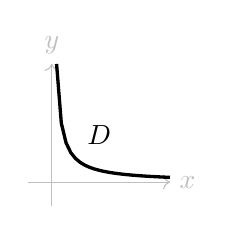
\begin{tikzpicture}[scale=0.6, domain=0.2:5]
\draw[] (1, 1) node {$D$};
\draw[color=lightgray, ->] (-0.5,0) -- (2.5,0) node[right] {$x$};
\draw[color=lightgray, ->] (0,-0.5) -- (0,2.5) node[above] {$y$};
\draw[color=black, very thick] plot (0.5*\x, 0.5/\x);
\end{tikzpicture}
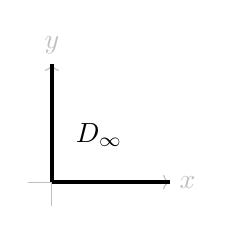
\begin{tikzpicture}[scale=0.6]
\draw[] (1, 1) node {$D_{\infty}$};
\draw[color=lightgray, ->] (-0.5,0) -- (2.5,0) node[right] {$x$};
\draw[color=lightgray, ->] (0,-0.5) -- (0,2.5) node[above] {$y$};
\draw[color=black, very thick] (0,0) -- (2.5,0);
\draw[color=black, very thick] (0,0) -- (0,2.5);
\end{tikzpicture}
\end{minipage}
\begin{minipage}[t]{0.1\textwidth}
\vspace{-30pt}
and
\end{minipage}
\begin{minipage}[t]{0.4\textwidth}
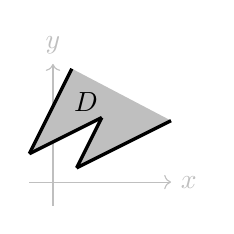
\begin{tikzpicture}[scale=0.6]
\draw[color=lightgray, ->] (-0.5,0) -- (2.5,0) node[right] {$x$};
\draw[color=lightgray, ->] (0,-0.5) -- (0,2.5) node[above] {$y$};
\fill[color=lightgray] (2.5,1.3) -- (0.5,0.3) -- (1.033333333,1.366666666) -- (-0.5,0.6) -- (0.4,2.4);
\draw[color=black, very thick] (0.5,0.3) -- (1.033333333,1.366666666);
\draw[color=black, very thick] (0.5,0.3) -- (2.5,1.3);
\draw[color=black, very thick] (-0.5,0.6) -- (0.4,2.4);
\draw[color=black, very thick] (-0.5,0.6) -- (1.033333333,1.366666666);
\draw[] (0.7, 1.7) node {$D$};
\end{tikzpicture}
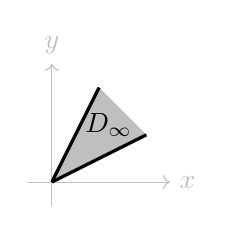
\begin{tikzpicture}[scale=0.6]
\draw[color=lightgray, ->] (-0.5,0) -- (2.5,0) node[right] {$x$};
\draw[color=lightgray, ->] (0,-0.5) -- (0,2.5) node[above] {$y$};
\fill[color=lightgray] (1,2) -- (0,0) -- (2, 1);
\draw[color=black, very thick] (0,0) -- (1,2);
\draw[color=black, very thick] (0,0) -- (2,1);
\draw[] (1.2, 1.2) node {$D_{\infty}$};
\end{tikzpicture}
\end{minipage}
\end{center}

\begin{lemma}[Asymptotic cone of a $\delta$-neighbourhood]
\label{lem.Asymptotic_cone_delt_neighb}
Let $D \subset V$ and let $\delta \in \RR$ with $\delta \geq 0$. Then
the $\delta$-neighbourhood of $D$
\[
D^{\delta} \coloneqq \set{x \in V}{\textrm{there is $y \in D$ with $\norm{x-y} \leq \delta$}}
\]
satisfies $(D^{\delta})_{\infty} = D_{\infty}$.
\end{lemma}

\begin{proof}[Proof of Lemma~\ref{lem.Asymptotic_cone_delt_neighb}]
We only have to show that $(D^{\delta})_{\infty} \subset D_{\infty}$. Let
$0 \neq x \in (D^{\delta})_{\infty}$ and let
$(x_i)_i$ be a sequence
in $D^{\delta}$ such that $\norm{x_i} \to \infty$ and $x_i / \norm{x_i} \to x / \norm{x}$.
By~definition,
there is a sequence $(y_i)_i$ in $D$ such that $\norm{x_i-y_i} \leq \delta$. In particular, we~get
$\norm{y_i} \to \infty$. Let $m_i \coloneqq \min\{\norm{x_i}, \norm{y_i}\}$. Then $m_i \to \infty$
and for sufficiently big~$i$
\[
0 \leq \norm{\frac{x_i}{\norm{x_i}}-\frac{y_i}{\norm{y_i}}} \leq \frac{\norm{x_i-y_i}}{m_i} \leq \frac{\delta}{m_i}.
\]
As $\sfrac{\delta}{m_i} \to 0$, the above inequality
implies
$\sfrac{x}{\norm{x}}\!=\!\lim_{i \to \infty} \sfrac{x_i}{\norm{x_i}}\!=\!\lim_{i \to \infty} \sfrac{y_i}{\norm{y_i}}$.
\end{proof}

For a subset $D \subset V$ we denote by $\inter(D)$ the topological interior
of $D$ inside the linear span of $D$.

\begin{lemma}[Intersection of a cone with an affine hyperplane.]
\label{lem.Intersection_with_affine_hyperplane}
Let $C \subset V$ be a cone and let $H_1$ be an affine hyperplane in $V$
such that $0 \not\in H_1$. If $C \cap H_1 \neq \varnothing$, then $\inter(C) \cap H_1 \neq \varnothing$.
\end{lemma}

\begin{proof}
Let $\pi \colon V \to \RR$ be a linear map such that $H_1 = \pi^{-1}(1)$.
By assumption, there is $c \in C \cap H_1$.
We may assume that $c$ lies in the topological boundary of $C$ inside the linear span of $C$
(otherwise we are finished).
By the continuity
of $\pi$, there is $c' \in \inter(C)$ such that $|\pi(c)- \pi(c')| < 1$. As $\pi(c) = 1$, we
get $\pi(c') > 0$. Then $\lambda = 1 / \pi(c') \in \RR_{> 0}$ and thus
$\lambda c' \in \inter(C) \cap H_1$.
\end{proof}

A subset $C \subset V$ is called \emph{convex} if for all
$x, y \in C$ and all $\alpha \in [0, 1]$, we have $\alpha x + (1- \alpha) y \in C$.
A convex cone $C \subset V$ is called \emph{strongly convex} if
it contains no linear subspace of $V$ except the zero subspace.
For a
subset $D \subset V$, we denote by $\Conv(D)$ the
\emph{convex cone generated by $D$} in $V$, \ie
\[
\Conv(D) = \set{\lambda_1 v_1 + \ldots + \lambda_k v_k \in V}{
\textrm{$v_1, \ldots, v_k \in D$ and $\lambda_1, \ldots, \lambda_k \in \RR_{\geq 0}$}}.
\]

\begin{lemma}[Asymptotic cone of the intersection of a closed convex
cone with an affine hyperplane]
\label{lem.Weights_facet_translated}
Let $C \subset V$ be a closed convex cone and let
$H \subset V$ be a hyperplane. Then for each $v \in V$ such that $C \cap (v+H) \neq \varnothing$, we have
\[
\left( C \cap (v+H) \right)_{\infty} = C \cap H.
\]
\end{lemma}

\begin{proof}
We denote $D \coloneqq C \cap (v+H) \subset V$. As
$D \neq \varnothing$ we can take $x \in D$. If~$y \in C \cap H$, then
$x+y \in C$ and $x+y \in v + H$, thus $x+y \in D$. This shows that
$x + (C \cap H) \subset D$ and by Lemma~\ref{lem.Properties_asymptotic_cone}, we get $C \cap H \subset D_\infty$.
Now, from Lemma~\ref{lem.Properties_asymptotic_cone} we get also the reverse inclusion
(here we use that $C$ is a closed cone):
\[
D_\infty = (C \cap (v+H))_\infty \subset C_\infty \cap (v+H)_\infty
= C_\infty \cap H_{\infty} = C \cap H.\qedhere
\]
\end{proof}

A subset $C\!\subset\!V$ is a \emph{convex polyhedral cone} if there is a finite subset
$F\!\subset\!V$ such~that
\[
C = \Conv F.
\]
For a convex polyhedral cone $C$ in $V$, set
\[
C^\vee = \set{x \in V}{\langle c, x \rangle\geq 0 \ \textrm{for all $c \in C$}}.
\]
By \cite[Propty\,(1), p.\,9]{Fu1993Introduction-to-to} we have $C = (C^\vee)^\vee$.
In particular $C$ is closed in $V$.

A hyperplane $H \subset V$ passing through the origin is called a \emph{supporting hyperplane} of a convex polyhedral cone
$C \subset V$ if
$C$ is contained in one of the closed half spaces in $V$
delimited by $H$, \ie there is a normal vector $u \in V$ to $H$
such that
\[
C \subset \set{x \in V}{\langle u, x \rangle\geq 0}.
\]
A \emph{face} of a convex polyhedral cone $C \subset V$ is the intersection of $C$ with a
supporting hyperplane of $C$ in $V$.
A face of dimension one of $C$ is called an \emph{extremal ray of $C$}.

For a fixed lattice $\Lambda \subset V$ (\ie a finitely generated subgroup of $(V, +)$ of rank $\dim V$),
a convex polyhedral cone $C \subset V$
is called \emph{rational (with respect to $\Lambda$)} if there is a finite subset $F \subset \Lambda$
such that $C = \Conv(F)$. In case $C$ is strongly convex, then~$C$ is rational if and only if
each extremal ray of $C$ is generated
by some element from $C \cap \Lambda$, see \cite[p.\,14]{Fu1993Introduction-to-to}.
Note that a face of a rational convex polyhedral cone
is again a rational convex polyhedral cone, see \cite[Prop.\,2]{Fu1993Introduction-to-to}.

\begin{lemma}
\label{lem.Weights_lattice}
Let $\Lambda \subset V$ be a lattice.
\begin{enumerate}
\item \label{lem.Weights_lattice_1} If $C \subset V$ is a rational convex
polyhedral cone, then $C = (C \cap \Lambda)_{\infty}$.
\item \label{lem.Weights_lattice_2} If $v_0 \in V$, $S \subset V$ denotes the unit sphere with center $0$ and
$\rho \colon V \setminus \{0\} \to S$ denotes the map given by $v \mto \sfrac{v}{\norm{v}}$,
then $\rho((v_0 + \Lambda) \setminus \{0\})$ is dense in $S$.
\end{enumerate}
\end{lemma}

\skpt
\begin{proof}
\eqref{lem.Weights_lattice_1}
Let $v_1, \ldots, v_r \in C \cap \Lambda$ such that $C = \Conv(v_1, \ldots, v_r)$. Then
\[
K\coloneqq\bset{\textstyle\sum_{i=1}^r t_i v_i \in V}{\textrm{$0 \leq t_i \leq 1$ for $i=1, \ldots, r$}}
\]
is a compact subset of $C$. In particular, there is a real number $\delta \geq 0$ such that
$\norm{v} \leq \delta$ for all $v \in K$. Now, let $c \in C$. Then there exist
$m_1, \ldots, m_r \in \ZZ_{\geq 0}$ and $0 \leq t_1, \ldots, t_r \leq 1$ such that
\[
c = \underbrace{\sum_{i=1}^r m_i v_i}_{\in C \cap \Lambda} +
\underbrace{\biggl(\sum_{i=1}^r t_i v_i \biggr)}_{\in K}.
\]
This shows that $c$ is contained in the $\delta$-neighbourhood $(C \cap \Lambda)^\delta$. In
summary, we get $C \cap \Lambda \subset C \subset (C \cap \Lambda)^\delta$ and by
using Lemmas~\ref{lem.Properties_asymptotic_cone} and~\ref{lem.Asymptotic_cone_delt_neighb}
the statement follows.

\eqref{lem.Weights_lattice_2}
By~\eqref{lem.Weights_lattice_1} applied to $C = V$ and
Lemma~\ref{lem.Properties_asymptotic_cone} we get
$V = \Lambda_{\infty} = (v_0 + \Lambda)_{\infty}$. By~definition of the asymptotic cone, thus
for every $v \neq 0$ in $V$ there exists a sequence $(\lambda_i)_i$ in $\Lambda$ such that
$\norm{v_0 + \lambda_i} \to \infty$ and
$\rho(v) = \lim_{i \to \infty} \rho(v_0 + \lambda_i)$.
This shows that $\rho((v_0 + \Lambda) \setminus \{0\})$ is dense in $S = \rho(V \setminus \{0\})$.
\end{proof}

\begin{proposition}
\label{prop.Weights_facet}
Let $\Lambda \subset V$ be a lattice, let $C \subset V$ be a convex polyhedral cone,
let $H \subset V$ be a hyperplane, and let $H' \coloneqq \gamma + H$ for some
$\gamma \in \Lambda \setminus H$.
\begin{enumerate}
\item
\label{prop.Weights_facet1}
If $C \cap H' \neq \varnothing$, $\dim C \cap H = \dim H$ and $H$ is rational, then
$\inter(C) \cap H' \cap \Lambda \neq \varnothing$.
\item
\label{prop.Weights_facet2}
If $\inter(C) \cap H' \cap \Lambda \neq \varnothing$ and
$C \cap H$ is a rational convex polyhedral cone, then
\[
C \cap H = (\inter(C) \cap H' \cap \Lambda)_{\infty}.
\]
\end{enumerate}
\end{proposition}

The pictures below illustrate the setups of Proposition~\ref{prop.Weights_facet} in the two
cases.
\begin{center}
\vspace*{-\baselineskip}
\begin{minipage}[t]{0.45\textwidth}
\[\tag{\ref{prop.Weights_facet1}}
\begin{array}{c}
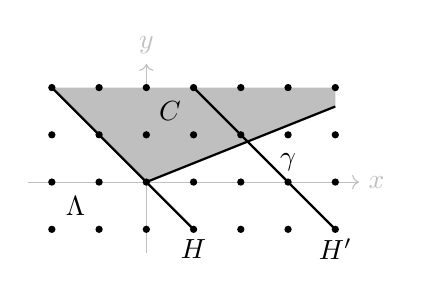
\begin{tikzpicture}[scale=0.6]
\draw[color=lightgray, ->] (-2.5,0) -- (4.5,0) node[right] {$x$};
\draw[color=lightgray, ->] (0,-1.5) -- (0,2.5) node[above] {$y$};
\fill[color=lightgray] (-2, 2) -- (0, 0) -- (4, 1.6) -- (4, 2);
\draw[color=black, thick] (1, -1) -- (-2, 2);
\draw[color=black, thick] (0, 0) -- (4, 1.6);
\draw[color=black, thick] (4, -1) -- (1, 2);
\foreach \i in {-2,...,4}
{
\foreach \j in {-1,...,2}
\fill[color=black] (\i, \j) circle [radius=2.2pt];

}
\draw[] (-1.5, -0.5) node {$\Lambda$};
\draw[] (0.5, 1.5) node {$C$};
\draw[] (1, -1) node[below] {$H$};
\draw[] (4, -1) node[below] {$H'$};
\draw[very thick] (3, 0) node[above] {$\gamma$};
\end{tikzpicture}
\end{array}
\]
\end{minipage}
\qquad
\begin{minipage}[t]{0.45\textwidth}
\[\tag{\ref{prop.Weights_facet2}}
\begin{array}{c}
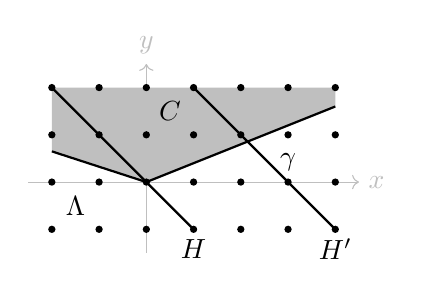
\begin{tikzpicture}[scale=0.6]
\draw[color=lightgray, ->] (-2.5,0) -- (4.5,0) node[right] {$x$};
\draw[color=lightgray, ->] (0,-1.5) -- (0,2.5) node[above] {$y$};
\fill[color=lightgray] (-2, 2) -- (-2, 0.65) -- (0, 0) -- (4, 1.6) -- (4, 2);
\draw[color=black, thick] (1, -1) -- (-2, 2);
\draw[color=black, thick] (0, 0) -- (-2, 0.65);
\draw[color=black, thick] (0, 0) -- (4, 1.6);
\draw[color=black, thick] (4, -1) -- (1, 2);
\foreach \i in {-2,...,4}
{
\foreach \j in {-1,...,2}
\fill[color=black] (\i, \j) circle [radius=2.2pt];

}
\draw[] (-1.5, -0.5) node {$\Lambda$};
\draw[] (0.5, 1.5) node {$C$};
\draw[] (1, -1) node[below] {$H$};
\draw[] (4, -1) node[below] {$H'$};
\draw[very thick] (3, 0) node[above] {$\gamma$};
\end{tikzpicture}
\end{array}
\]
\end{minipage}
\end{center}

\skpt
\begin{proof}
\eqref{prop.Weights_facet1}
If $\dim V = 1$, then $H = \{0\}$. Thus
$C \cap H' \neq \varnothing$ gives $C \cap H' = \{\gamma\} \subset \Lambda \setminus \{0\}$ and
the statement follows. Hence, we assume $\dim V \geq 2$.

As $\gamma \not\in H$, we get $0 \not\in H'$.
Since $C \cap H' \neq \varnothing$ there is thus $x \in \inter(C) \cap H'$
by~Lemma~\ref{lem.Intersection_with_affine_hyperplane}.
As $\dim(C \cap H) = \dim H$, the linear
span of $C \cap H$ is $H$ and we get that
$\inter(C \cap H)$ is a non-empty open subset of $H$. Set
\[
D \coloneqq x + (\inter(C\cap H) \setminus \{0\}) \subset (\inter(C) \cap H') \setminus \{x\}.
\]
Denote by $S$ the unit sphere in $H$ with center $0$ and consider
\[
\pi \colon H' \setminus \{x\} \to S, \quad w \mto \frac{w-x}{\norm{w-x}}.
\]
For all $h \in \inter(C \cap H)$ we have $\RR_{> 0}h \subset \inter(C \cap H)$ and thus
\[
\pi^{-1}(\pi(D)) = D.
\]
As $\dim H \geq 1$ (note that $\dim V \geq 2$), we get that $D$ is a non-empty open subset of $H' \setminus \{x\}$, and thus
the same is true
for $\pi(D)$ in $S$ (because $\pi$ is open). As
$\gamma \in \Lambda$ and $H' = \gamma + H$, it follows that
$H' \cap \Lambda = \gamma + (H \cap \Lambda)$. Using that $H$ is rational,
we get that
$\pi((H' \cap \Lambda) \setminus \{x\})$ is dense in $S$ by Lemma~\ref{lem.Weights_lattice}\eqref{lem.Weights_lattice_2} applied to the point $\gamma - x \in H$
and the lattice $H \cap \Lambda$ in $H$.
By the openness of $\pi(D)$ in $S$,
there is $\lambda \in (H' \cap \Lambda) \setminus \{x\} \subset \Lambda$
with $\pi(\lambda) \in \pi(D)$.
In particular, $\lambda \in \pi^{-1}(\pi(D)) = D$ and thus
$\lambda \in D \cap \Lambda \subset \inter(C) \cap H' \cap \Lambda$.

\eqref{prop.Weights_facet2} By assumption, there is $y \in \inter(C) \cap H' \cap \Lambda$. Thus
we get
\[
y + (C \cap H \cap \Lambda) \subset \inter(C) \cap H' \cap \Lambda.
\]
This implies by Lemma~\ref{lem.Properties_asymptotic_cone}
\[
\label{Eq:1}
\tag{a}
(C \cap H \cap \Lambda)_{\infty} \subset (\inter(C) \cap H' \cap \Lambda)_{\infty}
\subset (C \cap H')_{\infty}.
\]
By Lemma~\ref{lem.Weights_facet_translated} we get
\[
\label{Eq:2}
\tag{b}
(C \cap H')_{\infty} = C \cap H.
\]
By Lemma~\ref{lem.Weights_lattice}\eqref{lem.Weights_lattice_1}
applied to the rational convex polyhedral cone
$C \cap H \subset V$ we get
\[
\label{Eq:3}
\tag{c}
C \cap H = (C \cap H \cap \Lambda)_{\infty}.
\]
Combining~\eqref{Eq:1},~\eqref{Eq:2} and~\eqref{Eq:3} yields the result.
\end{proof}

\begin{proposition}
\label{prop.help_lemma_weights}
Let $\Lambda \subset V$ be a lattice, $C \subset V$ a
convex poly\-hedral cone and $H_0 \subset V$ a hyperplane such that
$C \cap H_0$ is a rational convex polyhedral cone. Let $H_1 \subset V$ be an affine hyperplane parallel to $H_0$ and
set $H_{-1} \coloneqq -H_1$.
If $C \cap H_i \neq \varnothing$ for each $i \in \{\pm1\}$, then
\[
C \cap H_{-1} \cap \Lambda \neq \varnothing \quad \iff \quad
C \cap H_1 \cap \Lambda \neq \varnothing.
\]
\end{proposition}

The picture below illustrates the setup of Proposition~\ref{prop.help_lemma_weights}.

\begin{center}
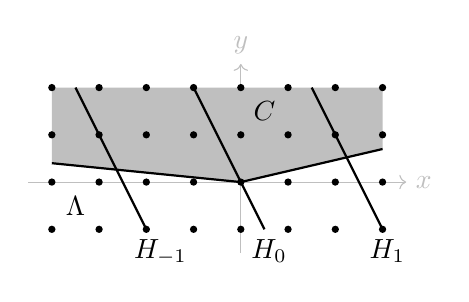
\begin{tikzpicture}[scale=0.6]
\draw[color=lightgray, ->] (-4.5,0) -- (3.5,0) node[right] {$x$};
\draw[color=lightgray, ->] (0,-1.5) -- (0,2.5) node[above] {$y$};
\fill[color=lightgray] (-4, 2) -- (-4, 0.4) -- (0, 0) -- (3, 0.7) -- (3, 2);
\draw[color=black, thick] (0.5, -1) -- (-1, 2);
\draw[color=black, thick] (3, -1) -- (1.5, 2);
\draw[color=black, thick] (-2, -1) -- (-3.5, 2);
\draw[color=black, thick] (0, 0) -- (3, 0.7);
\draw[color=black, thick] (0, 0) -- (-4, 0.4);
\foreach \i in {-4,...,3}
{
\foreach \j in {-1,...,2}
\fill[color=black] (\i, \j) circle [radius=2.2pt];

}
\draw[] (-3.5, -0.5) node {$\Lambda$};
\draw[] (0.5, 1.5) node {$C$};
\draw[] (-1.7, -1) node[below] {$H_{-1}$};
\draw[] (0.6, -1) node[below] {$H_0$};
\draw[] (3.1, -1) node[below] {$H_1$};
\end{tikzpicture}
\end{center}

\begin{proof}
If $H_0 = H_1$, then $H_0 = H_{-1}$ and the statement is trivial. Thus we assume that $H_0 \neq H_1$,
whence $H_0 \neq H_{-1}$ and $H_{1} \neq H_{-1}$.

Since $C \cap H_{\pm 1} \neq \varnothing$ and since $H_0$, $H_1$ and $H_{-1}$ are pairwise disjoint,
there exist $c_{\pm 1} \in \inter(C) \cap H_{\pm 1}$ by Lemma~\ref{lem.Intersection_with_affine_hyperplane}. As $C$ is convex, the line segment in
$V$ that connects~$c_1$ and~$c_{-1}$ lies in $\inter(C)$ and thus
$\inter(C) \cap H_0 \neq \varnothing$. Let
$B \subset C$ be the union of the proper faces of $C$, \ie $B$ is the topological
boundary of $C$ inside the linear span of~$C$, see \cite[Propty\,(7), p.\,10]{Fu1993Introduction-to-to}.
If $C \cap H_0 \cap \Lambda \subset B$, then by Lemma~\ref{lem.Weights_lattice}\eqref{lem.Weights_lattice_1} applied to
the rational convex polyhedral cone
$C \cap H_0$ in $V$ we get $C \cap H_0 = (C \cap H_0 \cap \Lambda)_{\infty} \subset B_{\infty} = B$,
a contradiction to $\inter(C) \cap H_0 \neq \varnothing$.
In particular, we may choose
\[
\gamma_0 \in (C \cap H_0 \cap \Lambda) \setminus B.
\]

By exchanging $H_1$ and $H_{-1}$, it is enough to prove
``$\Rightarrow$'' of the statement.
For this, let $\gamma_{-1} \in C \cap H_{-1} \cap \Lambda$.
Since $C$ is a convex polyhedral cone in $V$ (and thus in the linear span $\Span_{\RR}(C)$),
there is a finite set $E \subset \Span_{\RR}(C) \setminus \{0\}$ with
\[
C = \bigcap_{u \in E} \set{v \in \Span_{\RR}(C)}{\sprod{u}{v}\geq 0},
\]
see \cite[Propty\,(8), p. 11]{Fu1993Introduction-to-to}.
Since $\gamma_0 \in C \setminus B$, we get $\sprod{u}{\gamma_0} > 0$ for all $u \in E$. In~particular, we
may choose an integer $m \geq 0$ big enough so that
\[
\sprod{u}{m \gamma_0 - \gamma_{-1}} = m \sprod{u}{\gamma_0} - \sprod{u}{\gamma_{-1}} \geq 0
\]
for all $u \in E$, \ie $m \gamma_0 - \gamma_{-1} \in C$.
As $\gamma_0 \in H_0 \cap \Lambda$, we get
$m \gamma_0 - \gamma_{-1} \in C \cap H_1 \cap \Lambda$.
\end{proof}

\section{Quasi-affine varieties}
\label{sec.Quasi-affine}

To any variety $X$, we can naturally associate an affine scheme
\[
X_{\aff} \coloneqq \Spec \OO(X).
\]
Moreover this scheme comes equipped with the so-called canonical morphism
\[
\iota \colon X \to X_{\aff}
\]
which is induced by the natural isomorphism $\OO(X) = \OO(X_{\aff})$.

\begin{remark}
\label{rem.canonical_morphi_dominant}
For any variety $X$, the
canonical morphism $\iota \colon X \to X_{\aff}$ is dominant. Indeed, let
$X' \coloneqq \overline{\iota(X)} \subset X_{\aff}$ be the closure of the image of $\iota$
(endowed with the induced reduced subscheme structure).
Since the composition
\[
\OO(X) = \OO(X_{\aff}) \to \OO(X') \to \OO(X)
\]
is the identity on $\OO(X)$, it follows that the surjection $\OO(X)= \OO(X_{\aff}) \to \OO(X')$
is injective and thus $X' = X$.
\end{remark}

\begin{lemma}[{\cite[\S5, Prop.\,5.1.2]{Gr1961Elements-de-geomet-II}}]
\label{lem:Quasi-affine_irreducible}
Let $X$ be a variety. Then $X$ is quasi-affine if and only if the canonical morphism
$\iota \colon X \to X_{\aff}$ is an open immersion. \qed
\end{lemma}

If $X$ is quasi-affine and endowed with an algebraic group action, then this
action uniquely extends to an algebraic group action on $X_{\aff}$:

\begin{lemma}
\label{lem:Quasi-affine_group_action}
Let $X$ be a quasi-affine $H$-variety for some algebraic group $H$.
Then $X_{\aff}$ is an affine scheme that has a unique
$H$-action that extends the $H$-action on $X$ via the canonical open immersion
$X \hto X_{\aff}$.
\end{lemma}

\begin{proof}
By Lemma~\ref{lem:Quasi-affine_irreducible},
the canonical morphism $X \to X_{\aff}$
is an open immersion of schemes
and there is a unique action of $H$ on $X_{\aff}$ that extends the $H$-action on $X$, see
\eg \cite[Lem.\,5]{KrReSa2018Is-the-affine-spac}.
\end{proof}

Now, we compare the $G$-sphericity of $X$ and $X_{\aff}$.

\begin{lemma}
\label{lem:Spherical_quasi-affine}
Let $G$ be a connected reductive algebraic group and
let $X$ be a quasi-affine $G$-variety. Then
\[
\textrm{$X$ is $G$-spherical} \quad \iff \quad
\textrm{$X_{\aff}$ is an affine $G$-spherical variety}.
\]
\end{lemma}

\begin{proof}
If $X_{\aff}$ is an affine $G$-spherical variety, then $X$ is $G$-spherical by Lemma~\ref{lem:Quasi-affine_irreducible}.

For the other implication,
assume that $X$ is $G$-spherical. It follows that $\OO(X)$ is a
finitely generated algebra over the ground field
by \cite{Kn1993Uber-Hilberts-vier} and thus $X_{\aff} = \Spec \OO(X)$ is an affine variety.
Since $X$ is irreducible, $X_{\aff}$ is irreducible by Remark~\ref{rem.canonical_morphi_dominant}.
Moreover, for each $x \in X$, the local ring $\OO_{X, x}$ is integrally
closed and thus $\OO(X) = \bigcap_{x \in X} \OO_{X, x}$ is integrally closed,
\ie $X_{\aff}$ is normal. Since $X$ is an open subset of $X_{\aff}$,
and since a Borel subgroup of $G$ acts with an open orbit on $X$, the same is true
for $X_{\aff}$.
\end{proof}

For the rest in this section, we recall two classical facts from invariant theory.

\begin{proposition}[{see \cite[Lem.\,1.4, part\,II]{1994Algebraic-geometry} and \cite[\S2.4 Lem.]{Kr1984Geometrische-Metho}}]
\label{prop.locally_finite_and_rational}
Let $X$ be any variety endowed with an $H$-action for some
algebraic group $H$. The natural action of $H$ on $\OO(X)$ satisfies the following:
If $f \in \OO(X)$, then $\Span_{\kk}(Hf)$ is a finite dimensional $H$-invariant subspace
of $\OO(X)$ and $H$ acts regularly on it. \qed
\end{proposition}

\begin{proposition}[{see \cite[Th.\,3.3, part\,II]{1994Algebraic-geometry}}]
\label{prop:H-semi-invariants}
Let $H$ be a connected solvable alge\-braic group and let $X$ be an irreducible
quasi-affine $H$-variety. Then, for every $H$\nobreakdash-inva\-riant rational map
$f \colon X \dra \kk$ there exist $H$-semi-invariants $f_1, f_2 \in \OO(X)$
such that $f = f_1 / f_2$. \qed
\end{proposition}

\section{Vector fields}
\label{sec.vectorfields}

\subsection{Generalities on vector fields}
\label{sec.generalities_on_vectorfields}
Let $X$ be any variety. We denote by
$\Ve(X)$ the vector space of all
algebraic vector fields on $X$, \ie all algebraic sections of the tangent bundle
$T X \to X$. Note that $\Ve(X)$ is in a natural way an $\OO(X)$-module.

Now, assume $X$ is endowed with a regular action of an algebraic
group $H$. Then, $\Ve(X)$ is an $H$-module, via the following action: Let $h \in H$ and
$\xi \in \Ve(X)$, then $h \cdot \xi$ is defined via
\[
(h \cdot \xi) (x) = \mathrm{d} \varphi_h (\xi(\varphi_{h^{-1}}(x))) \quad \textrm{for each $x \in X$},
\]
where $\varphi_h$ denotes the automorphism of $X$ given by
multiplication with $h$ and $d\varphi_h$ denotes the differential of $\varphi_h$.
For a fixed character $\lambda \colon H \to \GG_m$ we say that a
vector field $\xi \in \Ve(X)$ is
\emph{normalized by $H$ with weight $\lambda$} if
$\xi$ is a $H$-semi-invariant of weight~$\lambda$,
\ie for all $h \in H$ the following diagram commutes
\[
\xymatrix{
TX \ar[rr]^{ \textrm{d} \varphi_h} && TX \\
X \ar[u]^{\xi} \ar[rr]^{\varphi_h} && X \ar[u]_{\lambda(h) \xi}
}
\]
We denote by $\Ve(X)_{\lambda, H}$
the subspace in $\Ve(X)$ of all vector fields which are normalized by $H$
with weight $\lambda$. If it is clear which action on $X$ is meant, we drop
the index $H$ and simply write $\Ve(X)_{\lambda}$. Note that $\Ve(X)_{\lambda}$
is in a natural way an $\OO(X)^H$-module, where $\OO(X)^H$
denotes the $H$-invariant regular functions on $X$.
We denote by $\Ve^H(X)$ the subspace of all
$H$-invariant vector fields in $\Ve(X)$, \ie $\Ve^H(X) = \Ve(X)_{0}$, where $0$
denotes the trivial character of $H$.

Now, assume that $X$ is affine. There is a $\kk$-linear map
\[
\Ve(X) \to \Der_{\kk}(\OO(X)), \quad \xi \mto D_{\xi},
\]
where $D_{\xi} \colon \OO(X) \to \OO(X)$ is given by $D_{\xi}(f)(x) \coloneqq \xi(x)(f)$
(here we identify the tangent space of $X$ at $x$ with the
$\kk$-derivations $\OO_{X, x}\to \kk$ in $x$). In fact, $\Ve(X) \to \Der_{\kk}(\OO(X))$ is an
isomorphism: Indeed, as $X$ is affine, we have
\[
\Ve(X) = \Bigset{ \eta \colon X \to TX }{
\begin{array}{l}
\textrm{$\eta$ is a set-theoretical section and for all $f \in \OO(X)$} \\
\textrm{the map $x \mto \eta(x)(f)$ is a regular function on $X$}
\end{array}
},
\]
see \cite[\S3.2]{FuKr2018On-the-geometry-of}.

\subsection{Homogeneous $\GG_\ra$-actions and vector fields}
\label{sec.GroupActionsAndVectorfields}

The material of this small subsection is contained in \cite[\S6.5]{FuKr2018On-the-geometry-of},
however formulated for all varieties.

Let $P$ be an algebraic group that acts regularly on a variety $X$.
Then we get a $\kk$-linear map $\Lie P \to \Ve(X)$,
$A \mto \xi_A$, where the vector field $\xi_A$ is given by
\[
\label{Eq:vectorfield_to_H-action}
\tag{$\varominus$}
\xi_A \colon X \to TX, \quad x \mto (\textrm{d}_e \mu_x) A
\]
and $\mu_x \colon P \to X$, $p \mto p x$ denotes the orbit morphism in $x$: Indeed~\eqref{Eq:vectorfield_to_H-action} is a morphism as it is the composition of the morphisms
\[
X \to T_e P \times TX, \ x \mto (A, 0_x) \quad \textrm{and} \quad
d \mu |_{T_e P \times TX} \colon T_e P \times TX \to TX,
\]
where $0_x \in TX$ denotes the zero vector inside $T_x X$ and
$\mu \colon P \times X \to X$ denotes the $P$-action.

\begin{lemma}
\label{lem.faithfull_action}
If $P$ is an algebraic group that acts faithfully on a variety $X$, then the
$\kk$-linear map $\Lie P \to \Ve(X)$, $A \mto \xi_A$ is injective.
\end{lemma}

\begin{proof}
For each $x \in X$, the kernel of the differential $\textrm{d}_e \mu_x \colon \Lie P \to T_x X$ of
the orbit morphism $\mu_x \colon P \to X$, $p \mto p x$ is equal to $\Lie P_x$, where
$P_x$ denotes the stabilizer of $x$ in $P$. If $A \in \Lie P$ satisfies $\xi_A = 0$, then
$(\textrm{d}_e \mu_x)A = 0$ for each $x \in X$, \ie $A \in \Lie P_x$ for each $x \in X$.
As $P$ acts faithfully on $X$, we get $\{e\} = \bigcap_{x \in X} P_x$ and thus
$\{0\} = \Lie( \bigcap_{x \in X} P_x ) = \bigcap_{x \in X} \Lie(P_ x)$ which implies $A = 0$.
\end{proof}

Let $H$ be an algebraic group. A $\GG_\ra$-action on an $H$-variety $X$ is called
\emph{$H$-homo\-geneous of weight $\lambda \in \mathfrak{X}(H)$} if
\[
h \circ \varepsilon(t) \circ h^{-1} = \varepsilon(\lambda(h) \cdot t) \quad
\textrm{for all $h \in H$ and all $t \in \GG_\ra$},
\]
where $\varepsilon \colon \GG_\ra \to \Aut(X)$ is the group homomorphism
induced by the $\GG_\ra$-action.

\begin{lemma}
\label{lem.H-homogeneous_Ga-action}
Let $H$ be an algebraic group, $X$ an $H$-variety and
$\rho$ an $H$-homo\-ge\-neous $\GG_\ra$-action on $X$
of weight $\lambda \in \mathfrak{X}(H)$. Then the image
of the previously introduced $\kk$\nobreakdash-linear map
$\Lie \GG_\ra \to \Ve(X)$, $A \mto \xi_A$ associated to $\rho$
lies in $\Ve(X)_{\lambda, H}$.
\end{lemma}

\begin{proof}
As $\rho$ is $H$-homogeneous, we get for each $x \in X$ and each $h \in H$
the following commutative diagram
\[
\xymatrix{
\GG_\ra \ar[d]_{\mu_x} \ar[rr]^-{t \mto \lambda(h) t} && \GG_\ra \ar[d]^-{\mu_{hx}} \\
X \ar[rr]^-{\varphi_h} && X
}
\]
where $\varphi_h \colon X \to X$ denotes multiplication by $h$. Taking differentials in the
neutral element $e \in \GG_\ra$
gives $\textrm{d}_x \varphi_h \textrm{d}_e \mu_x = \lambda(h) \textrm{d}_e \mu_{hx}$
for each $A \in \Lie \GG_\ra$. This implies that $h \cdot \xi_A(x) = \lambda(h) \xi_A(x)$
for each $A \in \Lie \GG_\ra$ and thus the statement follows.
\end{proof}

\begin{lemma}
\label{lem:D(X)_contained_in_the_weights_of_Ve^H(X)}
Let $H$ be an algebraic group and let $N \subset H$
be a normal subgroup such that the character group $\mathfrak{X}(N)$ is trivial.
If $X$ is an irreducible $H$-variety, then
\[
D_H(X) =
\Bigset{\lambda \in \mathfrak{X}(H)}{
\begin{array}{l}
\textrm{there is a non-trivial $H$-homogeneous} \\
\textrm{$\GG_\ra$-action on $X$ of weight $\lambda$}
\end{array}
}
\]
is contained in the set of $H$-weights of non-zero vector fields in $\Ve^{N}(X)$ that are normalized
by $H$.
\end{lemma}

\begin{proof}
Let $\rho \colon \GG_\ra \times X \to X$ be a non-trivial $\GG_\ra$-action on $X$.
By Lemmas~\ref{lem.faithfull_action} and~\ref{lem.H-homogeneous_Ga-action}
there is a non-zero $\xi \in \Ve(X)$ such that
for each $h \in H$ we have $h \cdot \xi = \lambda(h) \xi$.
Moreover, since $\mathfrak{X}(N) = 0$, $\xi$ is $N$-invariant.
Thus $D_H(X)$ is contained in the set of $H$-weights of non-zero vector fields in
$\Ve^{N}(X)$ that are normalized by $H$.
\end{proof}

Now, assume that $X$ is an affine variety and fix some non-zero element $A_0 \in \Lie \GG_\ra$.
Moreover, denote by $\LND_{\kk}(\OO(X)) \subset \Der_\kk(\OO(X))$ the cone of locally nilpotent derivations
on $\OO(X)$, \ie the cone in $\Der_\kk(\OO(X))$ of $\kk$-derivations $D$ of $\OO(X)$ such that
for all $f \in \OO(X)$ there is a $n = n(f) \geq 1$ such that $D^n(f) = 0$, where $D^n$ denotes the $n$-fold
composition of $D$. There is a map
\[
\{\textrm{$\GG_\ra$-actions on $X$}\} \stackrel{1:1}{\longleftrightarrow} \LND_{\kk}(\OO(X)), \quad \rho \mto D_{\xi_{A_0}},
\]
where $\xi_{A_0}$ is defined as in~\eqref{Eq:vectorfield_to_H-action} with respect to the $\GG_\ra$-action $\rho$. As for each $f \in \OO(X)$ we have that $D_{\xi_{A_0}}(f)$ is the morphism
$x \mto A_0(f \circ \mu_x)$ (we interpret $A_0$ as a $\kk$-derivation of $\OO_{\GG_\ra, e} \to \kk$ in $e$),
it follows from \cite[\S 1.5]{Fr2017Algebraic-theory-o} that the above map is in fact a bijection.

\subsection{Finiteness results on modules of vector fields}

Let $G$ be an algebraic group. For this subsection, let $X$ be a $G$-variety.
Note that $\Ve(X)$ is an
\emph{$\OO(X)$-$G$-module} via the $\OO(X)$- and $G$-module structures given in \S\ref{sec.generalities_on_vectorfields},
\ie $\Ve(X)$ is a $G$-module, it is an $\OO(X)$-module,
and both structures are compatible in the sense that
\[
g \cdot (f \cdot \xi) = (g \cdot f) \cdot (g \cdot \xi) \quad
\textrm{for all $g \in G$, $f \in \OO(X)$ and $\xi \in \Ve(X)$.}
\]

\begin{lemma}
\label{lem.finiteness_and_rationality_of_VecX}
Assume that $X$ is a quasi-affine $G$-variety and that $\OO(X)$ is finitely generated as a $\kk$-algebra.
Then the $\OO(X)$-$G$-module $\Ve(X)$ is finitely generated and rational,
\ie $\Ve(X)$ is finitely generated as an $\OO(X)$-module
and the $G$\nobreakdash-repre\-sentation $\Ve(X)$ is a sum of finite dimensional
rational $G$-subrepresentations.
\end{lemma}

\begin{proof}
Since $\OO(X)$ is finitely generated, $X_{\aff} = \Spec \OO(X)$ is an affine variety
that is endowed with a natural $G$-action, see Lemma~\ref{lem:Quasi-affine_group_action}. By
\cite[Satz\,2, II.2.S]{Kr1984Geometrische-Metho} there is a rational $G$-representation $V$ and a $G$-equivariant
closed embedding $X_{\aff} \subseteq V$. We~denote by
\[
\iota \colon X \to V
\]
the composition of the canonical open immersion $X \subset X_{\aff}$ with $X_{\aff} \subset V$.
Note that the image of $\iota$ is locally closed in $V$ and that $\iota$ induces
an isomorphism of $X$ onto that locally closed subset of $V$.
Thus, $\mathrm{d} \iota \colon T X \to T V |_X$ is a $G$-equivariant closed
embedding over $X$ which is linear on each fiber of $T X \to X$.
Thus we get an $\OO(X)$-$G$-module embedding
\[
\Ve(X) \to \Gamma(TV |_X), \quad
\xi \mto \mathrm{d} \iota \circ \xi,
\]
where $\Gamma(TV |_X)$ denotes the $\OO(X)$-$G$-module
of sections of $TV |_X \to X$. However, since the vector bundle
$TV |_X \to X$ is trivial, there is a
$\OO(X)$-$G$-module isomorphism
\[
\Gamma(TV |_X) \simeq \Mor(X, V),
\]
where $G$ acts on $\Mor(X, V)$ via $g \cdot \eta = (x \mto g\eta(g^{-1}x))$.
Now, the $\OO(X)$-$G$-module
$\Mor(X, V) \simeq \OO(X) \otimes_{\kk} V$ is finitely generated and
rational (see Proposition~\ref{prop.locally_finite_and_rational}),
and thus the statement follows.
\end{proof}

For the next result we recall the following definition.

\begin{definition}
Let $G$ be an algebraic group. A closed subgroup $H \subset G$
is called a \emph{Grosshans subgroup} if $G/H$ is quasi-affine and
$\OO(G/H) = \OO(G)^H$ is a finitely generated $\kk$-algebra.
\end{definition}

Let $G$ be a connected reductive algebraic group.
Examples of Grosshans subgroups of $G$ are unipotent radicals of parabolic
subgroups of $G$, see \cite[Th.\,16.4]{Gr1997Algebraic-homogene}.
In particular, the unipotent radical $U$ of a Borel subgroup
$B \subset G$ is a Grosshans subgroup in $G$
(see also \cite[Th.\,9.4]{Gr1997Algebraic-homogene}). A very important property of Grosshans subgroups is the following:

\begin{proposition}[{\cite[Th.\,9.3]{Gr1997Algebraic-homogene}}]
\label{prop:finite_generation_of_invariant}
Let $A$ be a finitely generated $\kk$-algebra and let~$G$
be a connected reductive algebraic group that acts via $\kk$-algebra automorphisms on~$A$
such that $A$ becomes a rational $G$-module.
If $H \subset G$ is a Grosshans subgroup, then the ring of $H$-invariants
\[
A^H = \set{a \in A}{\textrm{$h a = a$ for all $h \in H$}}
\]
is a finitely generated $\kk$-subalgebra of $A$. \qed
\end{proposition}

\begin{proposition}
\label{prop.MU_finitely_generated}
Let $R$ be a finitely generated $\kk$-algebra and assume
that a connected reductive algebraic group
$G$ acts via $\kk$-algebra automorphisms on $R$ such that
$R$ becomes a rational $G$-module. Let $H \subset G$ be a
Grosshans subgroup.
If $M$ is a finitely generated rational $R$-$G$-module,
then $M^H$ is a finitely generated $R^H$-module.
\end{proposition}

\begin{proof}
We consider the $\kk$-algebra $A = R \oplus \varepsilon M$, where the
multiplication on $A$ is defined via
\[
(r + \varepsilon m) \cdot (q + \varepsilon n) =
rq + \varepsilon (rn+qm).
\]
Since $R$ is a finitely generated $\kk$-algebra and since $M$
is a finitely generated $R$-module, $A$ is a finitely generated $\kk$-algebra.
Moreover, since $R$ and $M$ are rational $G$-modules,
$A$ is a rational $G$-module. Moreover,
$G$ acts via $\kk$-algebra automorphisms on $A$.
Since~$H$ is a Grosshans subgroup of $G$, it now follows
by Proposition~\ref{prop:finite_generation_of_invariant}
that
\[
A^H = R^H \oplus \varepsilon M^H
\]
is a finitely generated $\kk$-algebra. Thus one can choose
finitely many elements $m_1, \ldots, m_k \in M^H$
such that $\varepsilon m_1, \ldots, \varepsilon m_k$ generate $A^H$
as an $R^H$-algebra. However, since $\varepsilon^2 = 0$, it follows
that $m_1, \ldots, m_k$ generate $M^H$ as an $R^H$-module.

As $M$ is a rational $G$-module, it follows that $M^H$ is a rational $H$-module.
\end{proof}

As an application of Lemma~\ref{lem.finiteness_and_rationality_of_VecX} and
Proposition~\ref{prop.MU_finitely_generated} we get the following
finiteness result of $\Ve^{H}(X)$ for a Grosshans subgroup $H$ of a connected reductive
algebraic group.

\begin{corollary}
\label{cor.VecUX_finitely_generated}
Let $H$ be a Grosshans subgroup of a connected reductive algebraic group
$G$. If $X$ is a quasi-affine $G$-variety
such that $\OO(X)$ is finitely generated as a $\kk$-algebra, then
$\Ve^{H}(X)$ is a finitely generated $\OO(X)^{H}$-module. \qed
\end{corollary}

\subsection{Vector fields normalized by a group action with an open orbit}

For this subsection, let $H$ be an algebraic group and let $X$ be an irreducible
$H$-variety which contains an open $H$-orbit.
Moreover, fix a character $\lambda$ of $H$. We provide an upper bound on the dimension of
$\Ve(X)_\lambda = \Ve(X)_{\lambda, H}$.

\begin{lemma}
\label{lem:Normalized_Derivations}
Fix $x_0 \in X$ that lies in the open $H$-orbit and let $H_{x_0}$ be
the stabilizer of $x_0$ in $H$. Then, there exists an injection
of $\Ve(X)_\lambda$ into the $H_{x_0}$-eigenspace of the tangent space $T_{x_0} X$
of weight $\lambda |_{H_{x_0}}$ given by
\[
\xi \mto \xi(x_0).
\]
In particular, the dimension of $\Ve(X)_\lambda$ is smaller than or equal to the
dimension of the
$H_{x_0}$-eigenspace of weight $\lambda |_{H_{x_0}}$ of $T_{x_0} X$.
\end{lemma}

\begin{proof}
Let $\xi \in \Ve(X)_\lambda$. By definition we have for all $h \in H$
\[
\label{eq:equivariancy}
\tag{$\varobar$}
\lambda(h) \xi(hx_0) = \textrm{d} \varphi_h \xi(x_0),
\]
where $\varphi_h \colon X \to X$ denotes the automorphism given by
multiplication with $h$. Since~$x_0$ lies in the open $H$-orbit and $X$ is irreducible,
$\xi$ is uniquely determined by $\xi(x_0)$. Moreover,~\eqref{eq:equivariancy} implies that $\xi(x_0)$ is an
$H_{x_0}$-eigenvector of weight $\lambda |_{H_{x_0}}$ of $T_{x_0} X$.
\end{proof}

\section{Automorphism group of a variety and root subgroups}
\label{sec.AutomorphismGroups}

Let $X$ be a variety and denote by $\Aut(X)$ its automorphism group.
A subgroup $H \subset \Aut(X)$ is called an \emph{algebraic subgroup of $\Aut(X)$} if
$H$ has the structure of an algebraic group such that the
action $H \times X \to X$ is a regular action of the algebraic group $H$ on $X$. It follows from~\cite{Ra1964A-note-on-automorp} (see also \cite[Th.\,2.9]{KrReSa2018Is-the-affine-spac})
that this algebraic group structure on $H$ is unique in the following sense: if $H_1, H_2$ are algebraic
groups with group isomorphisms $\iota_i \colon H_i \to H$ for $i=1, 2$ such that
the induced actions $H_i \times X \to X$ are morphisms for $i=1, 2$, then
$\iota_2^{-1} \circ \iota_1 \colon H_1 \to H_2$ is an isomorphism of algebraic groups.

Let $X$, $Y$ be varieties.
We say that a group homomorphism $\theta \colon \Aut(X) \to \Aut(Y)$ \emph{preserves algebraic subgroups} if
for each algebraic subgroup $H \subset \Aut(X)$ its image $\theta(H)$ is an algebraic subgroup of $\Aut(Y)$
and if the restriction $\theta|_{H} \colon H \to \theta(H)$ is a homomorphism of algebraic groups.
We say that a group isomorphism $\theta \colon \Aut(X) \to \Aut(Y)$
\emph{preserves algebraic subgroups} if both
homomorphisms $\theta$ and $\theta^{-1}$ preserve algebraic subgroups.

Assume now that $X$ is an $H$-variety for some algebraic group $H$ and that
$U_0 \subset \Aut(X)$ is
a one-parameter unipotent subgroup, \ie an algebraic subgroup of $\Aut(X)$ that
is isomorphic to $\GG_\ra$. If for some isomorphism $\GG_\ra \simeq U_0$
of algebraic groups the induced $\GG_\ra$-action on $X$ is
$H$-homogeneous of weight $\lambda \in \mathfrak{X}(H)$, then we call
$U_0$ a \emph{root subgroup with respect to $H$
of weight $\lambda$} (see \S\ref{sec.GroupActionsAndVectorfields}). Note that this
definition does not depend on the choice of the isomorphism $\GG_\ra \simeq U_0$. This notion goes back
to \name{Demazure} \cite{De1970Sous-groupes-algeb}.

\begin{lemma}
\label{lem.auto_perserves_weights}
Let $X$, $Y$ be $H$-varieties for some algebraic group $H$.
If $\theta \colon \Aut(X) \to \Aut(Y)$ is a group homomorphism that
preserves algebraic subgroups and if $\theta$ is compatible with the $H$-actions
in the way that
\[
\xymatrix@=10pt{
& H \ar[ld] \ar[rd] & \\
\Aut(X) \ar[rr]^-{\theta} && \Aut(Y)
}
\]
commutes, then for any root subgroup $U_0 \subset \Aut(X)$ with respect to
$H$, the image $\theta(U_0)$ is either the trivial group or
a root subgroup with respect to $H$ of the same weight as $U_0$.
\end{lemma}

\begin{proof}
We can assume that $\theta(U_0)$ is not the trivial group.
Hence, $\theta(U_0)$ is a one-parameter unipotent group.

Let $\varepsilon \colon \GG_\ra \simeq U_0 \subset \Aut(X)$
be an isomorphism and let
$\lambda \colon H \to \GG_m$ be the weight of $U_0$. Then we have for each $t \in \GG_\ra$
\[
h \circ \theta(\varepsilon(t)) \circ h^{-1} =
\theta(h \circ \varepsilon(t) \circ h^{-1}) = \theta(\varepsilon(\lambda(h)\cdot t)).
\]
Since $\theta |_{U_0} \colon U_0 \to \theta(U_0)$ is a surjective
homomorphism of algebraic groups that are both isomorphic to $\GG_\ra$ (and since the ground field is of
characteristic zero), $\theta |_{U_0}$ is in fact an isomorphism.
Thus $\theta \circ \varepsilon \colon \GG_\ra \simeq \theta(U_0) \subset \Aut(X)$ is an isomorphism
and hence~$\lambda$ is the weight of $\theta(U_0)$ with respect to $H$.
\end{proof}

\section{Homogeneous \texorpdfstring{$\GG_\ra$}{Ga}-actions on quasi-affine toric varieties}
\label{sec.homogeneou_Ga-actions_quasi-affine}

In this section, we provide a description of the homogeneous $\GG_\ra$-actions
on a quasi-affine toric variety. Throughout this section, we denote by $T$ an algebraic torus.
Recall that a $T$-toric variety is a $T$-spherical variety.
A $\GG_\ra$-action is called
\emph{homogeneous} if it is $T$-homogeneous
of some weight $\lambda \in \mathfrak{X}(T)$, see~\S\ref{sec.GroupActionsAndVectorfields}.

Let $X$ be a toric variety. In case $X$ is affine, Liendo~\cite{Li2010Affine-Bbb-T-varie}
gave a full description
of all homogeneous $\GG_\ra$-actions. In case $X$ is quasi-affine, $X_{\aff} = \Spec(\OO(X))$ is an affine
$T$-toric variety by Lemma~\ref{lem:Spherical_quasi-affine}.
Moreover, every homogeneous $\GG_\ra$-action
on $X$ extends uniquely to a homogeneous $\GG_\ra$-action on $X_{\aff}$ by Lemma~\ref{lem:Quasi-affine_group_action}.
Thus we are led to the problem of describing the homogeneous $\GG_\ra$-actions on $X_{\aff}$ that preserve
the open subvariety $X$.

This requires some preparation.
First, we provide a description of $X_{\aff}$ in case $X$ is toric and
provide a characterization, when $X$ is quasi-affine. For this, let us introduce some basic terms
from toric geometry. As a reference we take~\cite{Fu1993Introduction-to-to} and~\cite{CoLiSc2011Toric-varieties}.

Note that $M = \mathfrak{X}(T) = \Hom_\ZZ(N, \ZZ)$, where $N$ denotes the free abelian group of rank
$\dim T$ of the regular group homomorphisms $\GG_m \to T$
and denote by $M_{\RR} = M \otimes_{\ZZ} \RR$, $N_{\RR} = N \otimes_{\ZZ} \RR$ the extensions to $\RR$.
Moreover, let
\[
M_{\RR} \times N_{\RR} \to \RR, \quad
(u, v) \mto \langle u, v \rangle
\]
be the canonical $\RR$-bilinear form. Denote by $\kk[M]$ the $\kk$-algebra with basis $\chi^m$ for all $m \in M$
and multiplication $\chi^m \cdot \chi^{m'} = \chi^{m+m'}$. Note that there is an identification
\[
T = \Spec \kk[M].
\]

Let $\sigma \subset N_{\RR}$ be a \emph{strongly convex rational
polyhedral cone} in $N_{\RR}$, \ie it is a convex rational polyhedral cone with respect to the lattice $N \subset N_{\RR}$ and $\sigma$ contains no non-zero linear subspace of $N_\RR$. Then its dual
\[
\sigma^\vee = \set{u \in M_{\RR}}{\textrm{$\langle u, v \rangle \geq 0$ for all $v \in \sigma$}}
\]
is a convex rational polyhedral cone in $M_\RR$.
Denote by $\sigma_M^\vee$ the intersection of $\sigma^\vee$ with~$M$ inside $M_{\RR}$.
We can associate to $\sigma$ a toric variety
\[
X_\sigma = \Spec \kk[\sigma_M^\vee], \quad \textrm{where} \quad
\kk[\sigma_M^\vee] = \bigoplus_{m \in \sigma_M^\vee} \kk \chi^m \subset \kk[M].
\]
The torus $T$ acts on $X_{\sigma}$ with an open orbit where this action is induced by the
coaction
$\kk[\sigma_M^\vee] \to \kk[\sigma_M^\vee] \otimes_{\kk} \kk[M]$,
$\chi^u \mto \chi^u \otimes \chi^u$. Note that we have an order-reversing
bijection between the faces of $\sigma$ and the faces of its dual $\sigma^\vee$:
\[
\{\textrm{faces of $\sigma$}\} \stackrel{1:1}{\longleftrightarrow}
\{\textrm{faces of $\sigma^\vee$}\}, \quad
\tau \mto \sigma^\vee \cap \tau^{\bot},
\]
where $\tau^\bot$ consists of those $u \in M_\RR$ that satisfy $\sprod{u}{v} = 0$ for all $v \in \tau$,
see \cite[Propty\,(10), p.\,12]{Fu1993Introduction-to-to}. Moreover, each face $\tau \subset \sigma$
determines an orbit of dimension \hbox{$n - \dim(\tau)$} of the $T$-action on $X_\sigma$ (see \cite[\S3.1]{Fu1993Introduction-to-to}).
We denote its closure in $X_\sigma$ by $V(\tau)$. In particular, $V(\tau)$ is an irreducible closed
$T$-invariant subset of $X_{\sigma}$.

More generally, for a fan $\Sigma$ of strongly convex rational polyhedral
cones in $N_{\RR}$ we denote by $X_\Sigma$ its
associated toric variety, which is covered by the open affine toric subvarieties $X_{\sigma}$,
where $\sigma$ runs through the cones in $\Sigma$.

\begin{lemma}
\label{lem.toric_qusi-affine}
Let $X = X_{\Sigma}$ be a toric variety for a fan $\Sigma$ of strongly convex rational
polyhedral cones in $N_{\RR}$. Denote by $\sigma_1, \ldots, \sigma_r \subset N_{\RR}$
the maximal cones in $\Sigma$ and set
\[
\sigma = \Conv \bigcup_{i=1}^r \sigma_i \subset N_{\RR}.
\]
Then:
\begin{enumerate}
\item \label{lem.toric_qusi-affine1} We have $X_{\aff} = X_\sigma$
and the canonical morphism $\iota \colon X \to X_{\aff}$
is induced by the embeddings $\sigma_i \subset \sigma$ for $i=1, \ldots, r$.\footnote{Note that we defined $X_{\sigma}$ only for strongly convex rational polyhedral
cones $\sigma$. However, the definition $X_{\sigma}$ makes sense for every convex rational polyhedral
cone $\sigma$. In this case, the torus $T$ may act non-faithfully on $X_\sigma$.}
\item \label{lem.toric_qusi-affine2}
The toric variety $X$ is quasi-affine if and only if each $\sigma_i$ is a face of $\sigma$.
Moreover, if $X$ is quasi-affine, then $\sigma$ is strongly convex.
\item \label{lem.toric_qusi-affine3}
If $X$ is quasi-affine, then the irreducible components of $X_{\aff} \setminus X$ are the
closed sets of the form $V(\tau)$, where $\tau$ is a minimal face of $\sigma$ with $\tau \not\in \Sigma$.
\item \label{lem.toric_qusi-affine4}
If $X$ is quasi-affine, then each face $\tau$ of $\sigma$ with $\tau \not\in \Sigma$
has dimension at least $2$. In particular,
$X_{\aff} \setminus X$ is a closed subset of codimension at least $2$
in $X_{\aff}$.
\end{enumerate}
\end{lemma}

Below we draw a picture where the fan $\Sigma$ with maximal cones $\sigma_1, \ldots, \sigma_4$
defines a $3$-dimensional quasi-affine variety with associated cone
$\sigma = \Conv \bigcup_{i=1}^4 \sigma_i$:\vspace*{5pt}

\begin{center}
\begin{minipage}[t]{0.3\textwidth}
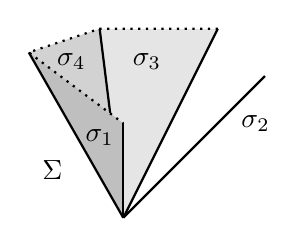
\begin{tikzpicture}[scale=0.6]
\fill[color=lightlightgray, thick, dotted] (2, 4) -- (0, 0) -- (-0.5, 4);
\fill[color=light1.5gray, thick, dotted] (-0.5, 4) -- (0, 0) -- (-2, 3.5);
\draw[color=black, thick] (0, 0) -- (2, 4);
\draw[color=black, thick] (0, 0) -- (-0.5, 4);
\fill[color=lightgray] (-2, 3.5) -- (0, 0) -- (0, 2);
\draw[color=black, thick] (0, 0) -- (-2, 3.5);
\draw[color=black, thick] (0, 0) -- (0, 2);
\draw[color=black, thick] (0, 0) -- (3, 3);
\draw[color=black, thick, dotted] (2, 4) -- (-0.5, 4) -- (-2, 3.5) -- (0, 2);
\draw[] (-1.5, 1) node {$\Sigma$};
\draw[] (-0.5, 1.7) node {$\sigma_1$};
\draw[] (2.8, 2) node {$\sigma_2$};
\draw[] (0.5, 3.3) node {$\sigma_3$};
\draw[] (-1.1, 3.3) node {$\sigma_4$};
\end{tikzpicture}
\end{minipage}
\begin{minipage}[t]{0.2\textwidth}
\phantom{and}
\end{minipage}
\begin{minipage}[t]{0.3\textwidth}
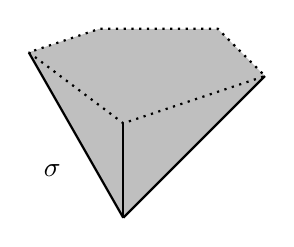
\begin{tikzpicture}[scale=0.6]
\fill[color=lightgray, thick, dotted] (-2, 3.5) -- (0, 0)-- (3, 3) -- (2, 4) -- (-0.5, 4);
\draw[color=black, thick, dotted] (-2, 3.5) -- (0, 2)-- (3, 3) -- (2, 4) -- (-0.5, 4) -- (-2, 3.5);
\draw[color=black, thick] (0, 0) -- (-2, 3.5);
\draw[color=black, thick] (0, 0) -- (0, 2);
\draw[color=black, thick] (0, 0) -- (3, 3);
\draw[] (-1.5, 1) node {$\sigma$};
\end{tikzpicture}
\end{minipage}
\end{center}

\skpt
\begin{proof}[Proof of Lemma~\ref{lem.toric_qusi-affine}]
\eqref{lem.toric_qusi-affine1}
Since the affine toric varieties $X_{\sigma_1}, \ldots, X_{\sigma_r}$
cover $X$, we get inside \hbox{$\OO(T)\!=\!\kk[M]$}:
\[
\OO(X) = \bigcap_{i=1}^r \OO(X_{\sigma_i}) =
\bigcap_{i=1}^r \kk[(\sigma_i)_M^{\vee}] =
\kk\biggl[ \biggl( \bigcap_{i=1}^r \sigma_i^{\vee} \biggr) \cap M \biggr].
\]
Since
\[
\sigma^\vee = \biggl(\Conv \bigcup_{i=1}^r \sigma_i\biggr)^\oldvee =
\set{u \in M_{\RR}}{\textrm{$\langle u, v \rangle \geq 0$ for all $v \in \sigma_i$ and all $i$}} =
\bigcap_{i=1}^r \sigma_i^\vee,
\]
we get $\OO(X) = \OO(X_\sigma)$ which implies the first claim.

For the second claim, denote by $\iota_i \colon X_{\sigma_i} \to (X_{\sigma_i})_{\aff}$
the canonical morphism of $X_{\sigma_i}$
(which is in fact an isomorphism). Then we have for each
$i=1, \ldots, r$ the commutative diagram
\[
\xymatrix@R=15pt{
X \ar[r]^-{\iota} & X_{\aff} \ar@{=}[r] & X_\sigma \\
X_{\sigma_i} \ar@{}[u] |-{\bigcup} \ar[r]^-{\iota_i} & (X_{\sigma_i})_{\aff} \ar[u]_-{\eta}
}
\]
where $\eta$ is induced by the inclusion $\kk[\sigma^{\vee}_M] \subset \kk[(\sigma_i)^\vee_M]$.
As $\eta \circ \iota_i \colon X_{\sigma_i} \to X_{\aff} = X_{\sigma}$
is induced by the inclusion $\sigma_i \subset \sigma$, the second claim follows.

\eqref{lem.toric_qusi-affine2}
If $\sigma_i \subset \sigma$ is a face, then
the induced morphism $X_{\sigma_i} \to X_{\sigma}$ is an open immersion
(see \cite[\S1.3 Lem.]{Fu1993Introduction-to-to}). Now, if each $\sigma_i$
is a face of $\sigma$, then by~\eqref{lem.toric_qusi-affine1} the canonical morphism
$\iota \colon X \to X_\sigma$ is an open immersion, \ie $X$ is quasi-affine (see Lemma~\ref{lem:Quasi-affine_irreducible}).

On the other hand, if $X$ is quasi-affine, then $\iota \colon X \to X_\sigma$ is an open immersion
(again by Lemma~\ref{lem:Quasi-affine_irreducible}) and by~\eqref{lem.toric_qusi-affine1}, the
morphism $X_{\sigma_i} \to X_{\sigma}$ induced by $\sigma_i \subset \sigma$
is also an open immersion. It now follows from
\cite[\S1.3 Exer.\,p.\,18]{Fu1993Introduction-to-to} that $\sigma_i$ is a face of $\sigma$.

If $X$ is quasi-affine, then $X_{\aff} = X_{\sigma}$ is a toric variety by Lemma~\ref{lem:Spherical_quasi-affine} and thus $\sigma$ is strongly convex.

\eqref{lem.toric_qusi-affine3}
We claim that $X_{\aff} \setminus X$ is the union
of all $V(\tau)$, where $\tau \subset \sigma$ is a face with $\tau \not\in \Sigma$.

Let $\tau \subset \sigma$ be a face such that
$\tau \not\in \Sigma$. In particular we have for all $i$ that $\tau \not\subset \sigma_i$.
Since $X$ is quasi-affine, $\sigma_i$ is a face of $\sigma$ by~\eqref{lem.toric_qusi-affine2}.
Hence, there is a $u_i \in \sigma^\vee_M$ with $u_i^\bot \cap \sigma = \sigma_i$ and
\[
X_{\sigma_i} = X_\sigma \setminus Z_{X_{\sigma}}(\chi^{u_i})
\]
by~\cite[\S1.3 Lem.]{Fu1993Introduction-to-to}, where $Z_{X_{\sigma}}(\chi^{u_i})$ denotes
the zero set of $\chi^{u_i} \in \OO(X_{\sigma})$ inside~$X_{\sigma}$.
As $\tau \subset \sigma$, but $\tau \not\subset \sigma_i$, we get
$\tau \not\subset u_i^\bot$ and thus $u_i \in \sigma_M^\vee \setminus \tau^\bot$.
By~\cite[\S3.1]{Fu1993Introduction-to-to}, the
closed embedding $V(\tau) \subset X_\sigma$ corresponds to the surjective $\kk$-algebra homomorphism
\[
\kk[\sigma^{\vee}_M] \to \kk[\sigma^{\vee}_M \cap \tau^{\bot}],
\quad
\chi^m \mto \begin{cases}
\chi^m & \textrm{if $m \in \tau^{\bot}$}, \\
0 & \textrm{if $m \in \sigma_M^\vee \setminus \tau^\bot$}.
\end{cases}
\]
In particular, $\chi^{u_i}$ vanishes on $V(\tau)$ and thus $V(\tau)$
and $X_{\sigma_i}$ are disjoint for all $i=1, \ldots, r$,
\ie $V(\tau) \subset X_{\aff} \setminus X$.
On the other hand, if $\eta \subset \sigma$ is a face with $\eta \in \Sigma$, then there is a
$i \in \{1, \ldots, r\}$ such that $\eta$ is a face of $\sigma_i$. Then by
\cite[\S3.1, p.\,53]{Fu1993Introduction-to-to},
it~follows that $V(\eta)$ and $X_{\sigma_i}$ do intersect. In particular,
$V(\eta) \not\subset X_{\aff} \setminus X$.
Since $X_{\aff} \setminus X$ is a closed $T$-invariant subset,
it is the union of some $V(\varepsilon)$ for some faces~$\varepsilon$ of~$\sigma$.
This implies then the claim.

Statement~\eqref{lem.toric_qusi-affine3} now follows from the claim,
since the minimal faces $\tau \subset \sigma$ with $\tau \not\in \Sigma$
correspond to the maximal $V(\tau)$ in $X_{\aff} \setminus X$.

\eqref{lem.toric_qusi-affine4}
Since $X$ is quasi-affine it follows from~\eqref{lem.toric_qusi-affine2}
that each $\sigma_i$ is a face of $\sigma$. Since $\sigma$ is the convex hull of the $\sigma_i$,
we get thus that the extremal rays of $\sigma$ are the same as the extremal rays of all the $\sigma_i$.
Hence the extremal rays of $\sigma$ are the same as the cones of dimension one in $\Sigma$. In particular,
each face $\tau$ of $\sigma$ with $\tau \not\in \Sigma$ has dimension at least~$2$.
\end{proof}

For the description of the homogeneous $\GG_\ra$-actions, let us set up the following notation. Let $\sigma \subset N_{\RR}$ be a strongly convex rational polyhedral cone.
If $\rho \subset \sigma$ is an extremal ray
and $\tau \subset \sigma$ a face, we denote
\[
\tau_\rho \coloneqq \Conv(\textrm{extremal rays in $\tau$ except $\rho$}) \subset N_{\RR}.
\]

In the picture below, we draw a picture of $\tau$ and $\tau_{\rho}$:\vspace*{5pt}
\begin{center}
\begin{minipage}[t]{0.3\textwidth}
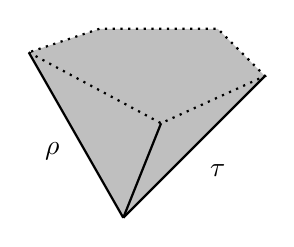
\begin{tikzpicture}[scale=0.6]
\fill[color=lightgray, thick, dotted] (-2, 3.5) -- (0, 0)-- (3, 3) -- (2, 4) -- (-0.5, 4);
\draw[color=black, thick, dotted] (-2, 3.5) -- (0.8, 2)-- (3, 3) -- (2, 4) -- (-0.5, 4) -- (-2, 3.5);
\draw[color=black, thick] (0, 0) -- (-2, 3.5);
\draw[color=black, thick] (0, 0) -- (0.8, 2);
\draw[color=black, thick] (0, 0) -- (3, 3);
\draw[] (2, 1) node {$\tau$};
\draw[] (-1.5, 1.4) node {$\rho$};
\end{tikzpicture}
\end{minipage}
\begin{minipage}[t]{0.2\textwidth}
\phantom{and}
\end{minipage}
\begin{minipage}[t]{0.3\textwidth}
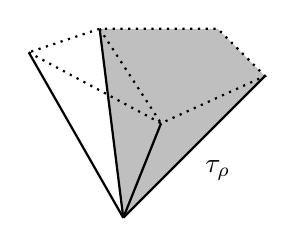
\begin{tikzpicture}[scale=0.6]
\fill[color=lightgray, thick, dotted] (0, 0)-- (3, 3) -- (2, 4) -- (-0.5, 4);
\draw[color=black, thick, dotted] (-2, 3.5) -- (0.8, 2)-- (3, 3) -- (2, 4) -- (-0.5, 4) -- (-2, 3.5);
\draw[color=black, thick, dotted] (-0.5, 4) -- (0.8, 2);
\draw[color=black, thick] (0, 0) -- (-0.5, 4);
\draw[color=black, thick] (0, 0) -- (-2, 3.5);
\draw[color=black, thick] (0, 0) -- (0.8, 2);
\draw[color=black, thick] (0, 0) -- (3, 3);
\draw[] (2, 1) node {$\tau_{\rho}$};
\end{tikzpicture}
\end{minipage}
\end{center}

In particular, if $\rho$ is not an extremal ray of $\tau$, then $\tau_\rho = \tau$. Let us mention the following
easy observations of this construction for future use:

\begin{lemma}
\label{lem.tau_rho_is_a_face}
Let $\sigma \subset N_{\RR}$ be a strongly convex rational polyhedral cone, $\tau \subset \sigma$
a face and $\rho \subset \sigma$ an extremal ray. Then
\begin{enumerate}
\item \label{lem.tau_rho_is_a_face1} $\tau_\rho$ is a face of $\sigma_\rho$;
\item \label{lem.tau_rho_is_a_face2} If $\dim \tau_\rho < \dim \tau $, then $\tau_\rho$ is a face of $\tau$.
\end{enumerate}
\end{lemma}

\skpt
\begin{proof}
\eqref{lem.tau_rho_is_a_face1}
By definition, there is $u \in \sigma^\vee$ with $\tau = \sigma \cap u^\bot$. Hence
$\tau_\rho \subset \sigma_\rho \cap u^\bot \subset \tau$. Since $u \in (\sigma_\rho)^\vee$,
$\sigma_\rho \cap u^\bot$ is a face of $\sigma_\rho$.
If $\rho \not\subset \tau$, then $\tau_\rho = \tau$
and thus $\tau_\rho = \sigma_\rho \cap u^\bot$ is a face of $\sigma_\rho$. If $\rho \subset \tau$,
then $\sigma_\rho \cap u^\bot$ is the convex cone generated by the extremal rays in $\tau$, except $\rho$, \ie $\tau_\rho = \sigma_\rho \cap u^\bot$. Thus $\tau_\rho$ is a face of $\sigma_\rho$.

\eqref{lem.tau_rho_is_a_face2}
As
$\dim \tau_\rho < \dim \tau$, we get $\rho \subset \tau$ and
\[
\label{eq.Span_tau}
\tag{$\boxbox$}
\Span_{\RR}(\tau) = \RR \rho \oplus \Span_{\RR}(\tau_\rho).
\]
Hence, there is $u \in M$ such that $\Span_{\RR}(\tau_\rho) = u^\bot \cap \Span_{\RR}(\tau)$.
After possibly replacing~$u$ by~$-u$, we may assume $\sprod{u}{v_\rho} \geq 0$, where
$v_\rho \in \rho$ denotes the unique primitive generator.
As $\tau_\rho \subset u^\bot$, we get now $u \in \tau^\vee$. Moreover,
\[
u^\bot \cap \tau = (u^\bot \cap \Span_{\RR}(\tau)) \cap \tau = \Span_{\RR}(\tau_\rho) \cap \tau = \tau_\rho,
\]
where the third equality follows from~\eqref{eq.Span_tau} as one may write
each element in $\tau$
as $\lambda v_{\rho} + \mu w$ for $w \in \tau_\rho$ and $\lambda, \mu \geq 0$.
Thus $\tau_\rho$ is a face of $\tau$.
\end{proof}

For each extremal ray $\rho$ in a strongly convex rational polyhedral cone $\sigma$, let
\[
S_{\rho} \coloneqq \set{w \in (\sigma_\rho)^\vee}{\sprod{w}{v_\rho} = -1} \cap M,
\]
where $v_\rho \in \rho$ denotes the unique primitive generator. In \cite[after Def.\,2.3]{Li2010Affine-Bbb-T-varie} there is an illuminating picture that shows the situation.
We provide below our own picture of the situation. In the first picture we draw $(\sigma_\rho)^\vee$
in light gray whereas in the second picture we draw $\sigma^\vee$ in light gray.\vspace*{5pt}

\begin{center}
\begin{minipage}[t]{0.3\textwidth}
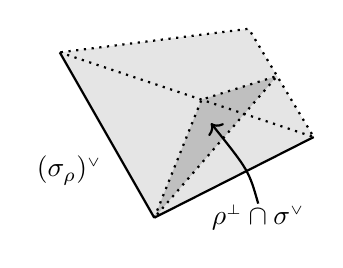
\begin{tikzpicture}[scale=0.6]
\fill[color=lightlightgray] (0, 0)-- (27/8, 1.70833) -- (2, 4) -- (-2, 3.5);
\draw[color=black, thick] (0, 0) -- (-2, 3.5);
\fill[color=lightgray] (0, 0) -- (1, 2.5) -- (2.6,3) -- (0, 0);
\draw[color=black, thick, thick, dotted] (0, 0) -- (1, 2.5) -- (2.6,3) -- (0, 0);
\draw[color=black, thick] (0, 0) -- (27/8, 1.70833);
\draw[color=black, thick, thick, dotted] (-2, 3.5) -- (27/8, 1.70833) -- (2, 4) -- (-2, 3.5);
\draw[] (-1.8, 1) node {$(\sigma_{\rho})^{\vee}$};
\draw[] (2.2, 0) node {$\rho^{\bot} \cap \sigma^{\vee}$};
\draw[color=black, thick, ->] (2.2, 0.3).. controls (2, 1).. (1.2,2);
\end{tikzpicture}
\end{minipage}
\qquad
\begin{minipage}[t]{0.5\textwidth}
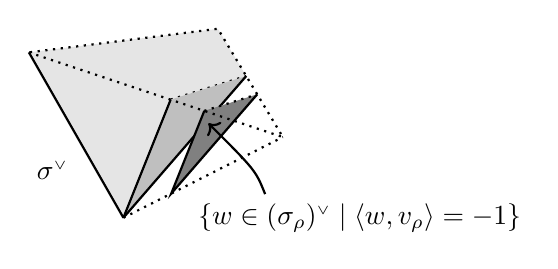
\begin{tikzpicture}[scale=0.6]
\fill[color=lightlightgray] (0, 0)-- (2.6, 3) -- (2, 4) -- (-2, 3.5);
\draw[color=black, thick, dotted] (1, 2.5) -- (2.6, 3);
\fill[color=lightgray] (0, 0) -- (1, 2.5) -- (2.6,3) -- (0, 0);
\draw[color=black, thick] (0, 0) -- (-2, 3.5);
\draw[color=black, thick] (0, 0) -- (1, 2.5);
\draw[color=black, thick] (0, 0) -- (2.6, 3);
\fill[color=gray] (1.7125, 2.2625) -- (1.0125, 0.512499) -- (2.8325, 2.6125);
\draw[color=black, thick] (1.7125, 2.2625) -- (1.0125, 0.512499) -- (2.8325, 2.6125);
\draw[color=black, thick, dotted] (1.7125, 2.2625) -- (2.8325, 2.6125);
\draw[color=black, thick, dotted] (-2, 3.5) -- (27/8, 1.70833) -- (2, 4) -- (-2, 3.5);
\draw[color=black, thick, dotted] (0, 0) -- (27/8, 1.70833);
\draw[] (-1.5, 1) node {$\sigma^{\vee}$};
\draw[] (5, 0) node {$\set{w \in (\sigma_\rho)^\vee}{\sprod{w}{v_\rho} = -1}$};
\draw[color=black, thick, ->] (3, 0.5).. controls (2.8, 1).. (1.8,2);
\end{tikzpicture}
\end{minipage}
\end{center}

\begin{remark}[{see also \cite[Rem.\,2.5]{Li2010Affine-Bbb-T-varie}}]
\label{rem.S_rho_non-empty}
The set $S_\rho$ is non-empty. Indeed, apply Proposition~\ref{prop.Weights_facet}\eqref{prop.Weights_facet1}
to the convex polyhedral cone $C = \sigma_\rho^\vee$ and the hyperplanes $H = \rho^\bot$,
$H' = \set{u \in M_\RR}{\sprod{u}{v_\rho} = -1}$
inside $V = M_\RR$.
\end{remark}

Now, we come to the promised description
of the homogeneous $\GG_\ra$-actions on toric varieties due to \name{Liendo}:

\begin{proposition}[{\cite[Lem.\,2.6, Th.\,2.7]{Li2010Affine-Bbb-T-varie}}]
\label{prop.G_a-actions_on_affine_toric_var}
Let $\sigma \subset N_\RR$ be a strongly convex rational polyhedral cone.
Then for any extremal ray $\rho$ in $\sigma$ and any
$e \in S_\rho$, the $\kk$-linear map
\[
\partial_{\rho, e} \colon \kk[\sigma^\vee_M] \to \kk[\sigma^\vee_M]
, \quad
\chi^m \mto \langle m, v_\rho \rangle \chi^{e+m}
\]
is a homogeneous locally nilpotent derivation of degree $e$,
and every homogeneous locally nilpotent derivation of $\kk[\sigma^\vee_M]$
is a constant multiple of some $\partial_{\rho, e}$. \qed
\end{proposition}

\begin{remark}
The weight of the homogeneous $\GG_\ra$-action induced by $\partial_{\rho, e}$ is $e \in M$.
The kernel of the locally nilpotent derivation $\partial_{\rho, e}$ is $\kk[\sigma_M^\vee \cap \rho^\bot]$.
\end{remark}

The following lemma is the key for the description of the homogeneous $\GG_\ra$-actions on a
quasi-affine toric variety.

\begin{proposition}
\label{Prop:Orbit_closure_invariant}
Let $\sigma \subset N_{\RR}$ be a strongly convex rational polyhedral cone, $\tau \subset \sigma$ a face,
$\rho \in \sigma$ an extremal ray and $e \in S_\rho$. Then the
$\GG_\ra$-action on $X_\sigma$ corresponding to the locally nilpotent derivation $\partial_{\rho, e}$
leaves $V(\tau)$ invariant if and only if
\[
\rho \not\subset \tau \quad \textrm{or} \quad e \not\in \tau_{\rho}^\bot.
\]
\end{proposition}

\begin{proof}
As in the proof of~Lemma~\ref{lem.toric_qusi-affine}~\eqref{lem.toric_qusi-affine3},
the embedding
$\iota \colon V(\tau) \subset X_\sigma$ corresponds to the surjective $\kk$-algebra homomorphism
\[
\iota^\ast \colon \kk[\sigma^{\vee}_M] \to \kk[\sigma^{\vee}_M \cap \tau^{\bot}],
\quad
\chi^m \mto \begin{cases}
\chi^m & \textrm{if $m \in \tau^{\bot}$}, \\
0 & \textrm{if $m \in \sigma_M^\vee \setminus \tau^\bot$}.
\end{cases}
\]
Thus the $\GG_\ra$-action on $X_\sigma$ corresponding to $\partial_{\rho, e}$
preserves $V(\tau)$ if and only
if
\[
\partial_{\rho, e}(\ker \iota^\ast) \subset \ker \iota^\ast,
\]
see \cite[\S 1.5]{Fr2017Algebraic-theory-o}.
Since $\sprod{m}{v_\rho} = 0$ for all $m \in \rho^\bot$
and since $e + m \in \sigma^\vee_M$ for all $m \in \sigma^\vee_M \setminus \rho^\bot$,
this last condition is equivalent to
\[
\label{Eq:Condition_Invariant}
\tag{$\odot$}
m \in \sigma_M^\vee \setminus (\tau^\bot \cup \rho^\bot) \quad \implies \quad
e+m \not\in \tau^\bot.
\]
We now distinguish two cases:
\begin{enumerate}
\item Assume $\rho \not\subset \tau$. Then $\tau \subset \sigma_\rho$. In particular, we
get $\sprod{e}{v} \geq 0$ for all $v \in \tau$.
Let $m \in \sigma_M^\vee \setminus \tau^\bot$. Then
we get $\sprod{m}{v} > 0$ for some $v \in \tau$ and hence
\[
\sprod{e+m}{v} > 0 \quad \textrm{for some $v \in \tau$},
\]
which in turn implies $e + m \not\in \tau^\bot$. Thus
\eqref{Eq:Condition_Invariant} is satisfied.
\item Assume $\rho \subset \tau$. In particular, we have $\tau^\bot \subset \rho^\bot$.
We distinguish two cases:
\begin{itemize}
\item $e \not\in \tau_{\rho}^\bot$: Then there exists an
extremal ray $\rho' \subset \tau$ with $\rho' \neq \rho$ such that $e \not\in (\rho')^\bot$ and
the unique primitive generator
$v_{\rho'} \in \rho'$ satisfies
\[
\sprod{e+m}{v_{\rho'}} = \underbrace{\sprod{e}{v_{\rho'}}}_{>0} + \underbrace{\sprod{m}{v_{\rho'}}}_{\geq 0}
> 0 \quad \textrm{for all $m \in \sigma_M^\vee$}.
\]
In particular $e+m \not\in \tau^\bot$
for all $m \in \sigma_M^\vee$ and thus~\eqref{Eq:Condition_Invariant} is satisfied.

\item $e \in \tau_\rho^\bot$:
Now, we want to apply Proposition~\ref{prop.help_lemma_weights}.
For this we fix the lattice $\Lambda = M \cap \tau_{\rho}^\bot$ inside
$V = \tau_{\rho}^\bot$.
Since $\tau_\rho$ is a face of $\sigma_\rho$ (see Lemma~\ref{lem.tau_rho_is_a_face}\eqref{lem.tau_rho_is_a_face1}),
$C =(\sigma_\rho)^\vee \cap \tau_{\rho}^\bot$ is a rational convex polyhedral cone
in $M_\RR$ and thus also in $V$.
Moreover, we set $H_0 = \rho^\bot \cap V = \tau^\bot$
and $H_{\pm1} = \set{u \in V}{\sprod{u}{v_{\rho}} = \pm 1}$.
Since $e \in (S_\rho \cap \tau_\rho^\bot) \setminus H_0$, $H_0$ is a hyperplane in $V$ and
$C \cap H_{-1} \cap \Lambda = S_{\rho} \cap \tau_{\rho}^\bot \neq \varnothing$.
Since $H_0 \subsetneq V$ we get thus $\dim \tau_\rho < \dim \tau$.
Now, by Lemma~\ref{lem.tau_rho_is_a_face}\eqref{lem.tau_rho_is_a_face2},
$\tau_\rho$ is a face of~$\tau$ and therefore
$\sigma^\vee \cap \tau_\rho^\bot \supsetneq \sigma^\vee \cap \tau^\bot$
by the order-reversing bijection between faces of $\sigma$ and
$\sigma^\vee$. Hence,
there is $u \in (\sigma^\vee \cap \tau_\rho^\bot) \setminus \tau^\bot$ and in particular
$u \in C \setminus H_0$. As~$\sprod{u}{v_{\rho}} > 0$, after scaling $u$
with a real number $>0$, we may assume
$u \in C \cap H_1$ and hence $C \cap H_1 \neq \varnothing$.
Now, as $C \cap H_0 = \sigma^\vee \cap \tau^{\bot}$ is rational
in $M_{\RR}$ and thus also in $V$,
we may apply Proposition~\ref{prop.help_lemma_weights} and get an element
\[
m_1 \in (\sigma_\rho)^\vee \cap \tau_{\rho}^\bot \cap \set{m \in M}{\sprod{m}{v_{\rho}}=1}.
\]
Hence, $m_1 \in \sigma_M^\vee \setminus \rho^\bot$.
Since $e, m_1 \in \tau_{\rho}^\bot$, we get
$e + m_1 \in \tau_{\rho}^\bot$. Since
\[
\sprod{e + m_1}{v_{\rho}} = \sprod{e}{v_{\rho}} + \sprod{m_1}{v_{\rho}} = -1 + 1 = 0,
\]
we get thus $e + m_1 \in \tau^\bot$. This implies
that~\eqref{Eq:Condition_Invariant} is not satisfied.\qedhere
\end{itemize}
\end{enumerate}
\end{proof}

We can use this lemma to provide a full description of all homogeneous $\GG_\ra$-actions on a quasi-affine toric variety $X = X_\Sigma$.
Recall that $X_{\aff} = X_\sigma$, where $\sigma$ is the
cone in\,$N_{\RR}$ generated by all maximal cones in $\Sigma$, see
Lemma~\ref{lem.toric_qusi-affine}. Moreover, $X_{\aff} \setminus X$ is the union of the
sets of the form $V(\tau)$, where $\tau \subset \sigma$ runs through the minimal faces with
the property that $\tau \not\in \Sigma$ (again by Lemma~\ref{lem.toric_qusi-affine}).
In the next corollaries (Corollary~\ref{Cor:Classification_LND_Quasi-affine}- Corollary~\ref{cor.DX_generates_M_as_a_group}),
we use this notation freely.

\begin{corollary}
\label{Cor:Classification_LND_Quasi-affine}
Let $X = X_{\Sigma}$ be a quasi-affine toric variety, let $X_{\aff} = X_\sigma$ and let $\tau_1, \ldots, \tau_s \subset \sigma$
be the minimal faces of $\sigma$ which do not belong to $\Sigma$. Then, the homogeneous
$\GG_\ra$-actions on $X$ are the restricted homogeneous $\GG_\ra$-actions on $X_{\aff}$ that
are induced by the constant multiples of $\partial_{\rho, e} \in \LND_{\kk}(\OO(X))$
such that
for all $i = 1, \ldots, s$ we have
\[
\label{Eq:Classification_LND_Quasi-affine}
\tag{$\circledast$}
\rho \not\subset \tau_i \quad \textrm{or} \quad e \not\in (\tau_i)_{\rho}^\bot.
\]
\end{corollary}

\begin{proof}
Assume that $\partial_{\rho, e}$ is a locally nilpotent derivation of $\OO(X)$
such that~\eqref{Eq:Classification_LND_Quasi-affine} is satisfied for all $i =1, \ldots, s$.
Then by Proposition~\ref{Prop:Orbit_closure_invariant}, the sets $V(\tau_1), \ldots, V(\tau_s) \subset X_{\aff}$
are left invariant by the homogeneous $\GG_\ra$-action
$\varepsilon_{\rho, e} \colon \GG_\ra \times X_{\aff} \to X_{\aff}$
which is induced by $\partial_{\rho, e}$.
In particular, $X = X_{\aff} \setminus (V(\tau_1) \cup \ldots V(\tau_s))$ (see Lemma~\ref{lem.toric_qusi-affine}) is left
invariant by $\varepsilon_{\rho, e}$.

On the other hand, let $\varepsilon \colon \GG_\ra \times X \to X$ be a homogeneous $\GG_\ra$-action on $X$.
By Lemma~\ref{lem:Quasi-affine_group_action} and Proposition~\ref{prop.G_a-actions_on_affine_toric_var}
this $\GG_\ra$-action extends to a homogeneous $\GG_\ra$-action
$\varepsilon_{\rho, e} \colon \GG_\ra \times X_{\aff} \to X_{\aff}$ which is induced
by some locally nilpotent derivation $\lambda \cdot \partial_{\rho, e} \in \LND_{\kk}(\OO(X))$ for some
constant $\lambda \in \kk$, some
extremal ray $\rho$ in $\sigma$ and some $e \in S_{\rho}$. Since $\varepsilon_{\rho, e}$ extends
$\varepsilon$, the subset $V(\tau_1) \cup \ldots \cup V(\tau_s) = X_{\aff} \setminus X$ is left
invariant by $\varepsilon_{\rho, e}$. Since the $V(\tau_1), \ldots, V(\tau_s)$ are the
irreducible components of $X_{\aff} \setminus X$ and since~$\GG_\ra$ is an irreducible algebraic group, it follows that $\varepsilon_{\rho, e}$ preserves each $V(\tau_i)$.
By~Proposition~\ref{Prop:Orbit_closure_invariant} we get that for each $i=1, \ldots, s$
the condition~\eqref{Eq:Classification_LND_Quasi-affine} is satisfied.
\end{proof}

For the next consequences of Corollary~\ref{Cor:Classification_LND_Quasi-affine} we recall the
following notation from Section~\ref{sec.Cones_and_asymptotic_cones}: For a
subset $E \subset M_{\RR}$ we denote by $\inter(E)$ the topological interior of $E$
inside the linear span of $E$. In these consequences we provide a closer
description of the weights in $M$ arising from homogeneous $\GG_\ra$-actions on quasi-affine toric varieties
and compute the asymptotic cone of these weights.

\begin{corollary}
\label{cor.Weights_rho}
Let $X = X_{\Sigma}$ be a quasi-affine toric variety, let $X_{\aff}=X_{\sigma}$, let
$\rho \subset \sigma$ be an extremal ray and let $D_{\rho}(X)$
be the set of weights $e \in S_\rho$ such that the locally nilpotent derivation
$\partial_{\rho, e}$ of $\OO(X)$ induces a homogeneous $\GG_\ra$-action on $X$. Then
\[
S_{\rho} \cap \inter(\sigma_{\rho}^\vee) \subset
D_{\rho}(X) \subset S_\rho.
\]
\end{corollary}

\begin{proof}
Let $e \in S_{\rho} \subset M$ such that $e$ is contained in
$\inter(\sigma_{\rho}^\vee) \subset M_{\RR}$.
Let $\tau_1, \ldots, \tau_s$ be the minimal faces of $\sigma$ which are not contained in $\Sigma$.
According to Corollary~\ref{Cor:Classification_LND_Quasi-affine} it is enough to show that for each $\tau_i$
with $\rho \subset \tau_i$ we have $e \not\in (\tau_i)_{\rho}^\bot$. By
Lemma~\ref{lem.toric_qusi-affine}~\eqref{lem.toric_qusi-affine4} we get that $\dim \tau_i \geq 2$
for every $i$. Hence, $\dim (\tau_i)_\rho \geq 1$
and thus $(\tau_i)_\rho^\bot \cap \sigma_\rho^\vee$ is a proper face of $\sigma_\rho^\vee$. As
$e \in \inter(\sigma_\rho^\vee)$, we get
$e \not\in (\tau_i)_\rho^\bot \cap \sigma_\rho^\vee$ and thus $e \not\in (\tau_i)_\rho^\bot$.
\end{proof}

\begin{corollary}
\label{cor.Weights}
Let $X = X_\Sigma$ be a quasi-affine toric variety. Let $X_{\aff} = X_{\sigma}$
and let $D(X)$ be the set of homogeneous $\GG_\ra$-weights on $X$.
Then the asymptotic cone of
$D(X) \subset M_{\RR}$ satisfies
\[
D(X)_{\infty} = \sigma^\vee \setminus \inter(\sigma^\vee).
\]
\end{corollary}

By Corollary~\ref{cor.Weights_rho}, the set $D(X)$ is contained in
the set
\[
S \coloneqq \bigcup_{\substack{
\textrm{$\rho$ is an extr.} \\
\textrm{ray of $\sigma$}
}} \set{w \in (\sigma_\rho)^\vee}{\sprod{w}{v_\rho} = -1}.
\]
Below, we illustrate the dual cone of $\sigma$ in light gray
and the set $S$ associated to $\sigma$ in dark gray:

\begin{center}
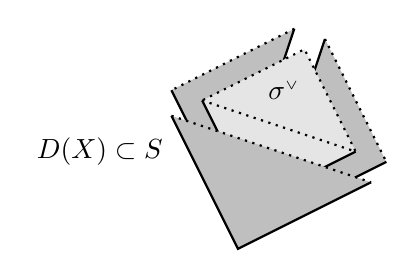
\begin{tikzpicture}[scale=0.65]
\fill[color=lightgray] (1.4, 3.2) -- (0.2, -0.4) -- (2.6, 0.8);
\draw[color=black, thick] (1.4, 3.2) -- (0.2, -0.4) -- (2.6, 0.8);
\draw[color=black, thick, dotted] (1.4, 3.2) -- (2.6, 0.8);

\fill[color=lightgray] (0.8, 3.4) -- (-0.4, -0.2) -- (-1.6, 2.2);
\draw[color=black, thick] (0.8, 3.4) -- (-0.4, -0.2) -- (-1.6, 2.2);
\draw[color=black, thick, dotted] (0.8, 3.4) -- (-1.6, 2.2);

\fill[color=lightlightgray] (-1, 2) -- (0, 0) -- (2, 1) -- (1, 3);
\draw[color=black, thick, dotted] (-1, 2) -- (2, 1) -- (1, 3) -- (-1, 2);
\draw[color=black, thick] (0, 0) -- (-1, 2);
\draw[color=black, thick] (0, 0) -- (2, 1);

\fill[color=lightgray] (-1.6, 1.7) -- (-0.3, -0.9) -- (2.3, 0.4);
\draw[color=black, thick] (-1.6, 1.7) -- (-0.3, -0.9) -- (2.3, 0.4);
\draw[color=black, thick, dotted] (-1.6, 1.7) -- (2.3, 0.4);

\draw[] (0.6, 2.2) node {$\sigma^{\vee}$};
\draw[] (-3, 1)
node {$D(X) \subset S$};
\end{tikzpicture}
\end{center}
Intuitively (and rigorously with Lemma~\ref{lem.Weights_facet_translated} applied to the
convex polyhedral cone $(\sigma_\rho)^{\vee}$ and the hyperplane $\rho^{\bot}$
for each $\rho$) it follows that
the asymptotic cone of $D(X)$
is contained in $\bigcup_{\rho} \set{w \in (\sigma_\rho)^\vee}{\sprod{w}{v_\rho} = 0}$.
This last set is equal to $\sigma^{\vee} \setminus \inter(\sigma^{\vee})$. Now, we provide a detailed proof.

\begin{proof}
By \cite[Propty\,(7), p.\,10]{Fu1993Introduction-to-to} we have
\[
\sigma^\vee \setminus \inter(\sigma^\vee) = \bigcup_{\substack{
\textrm{$\rho$ is an extr.} \\
\textrm{ray of $\sigma$}
}} \sigma^\vee \cap \rho^\bot.
\]
Since $D(X)$ is the union of the $D_{\rho}(X)$ for the extremal rays $\rho \subset \sigma$
(with the definition of $D_\rho(X)$ from Corollary~\ref{cor.Weights_rho}),
we get by Lemma~\ref{lem.Properties_asymptotic_cone} that
\[
D(X)_{\infty} = \bigcup_{\substack{
\textrm{$\rho$ is an extr.} \\
\textrm{ray of $\sigma$}
}} D_{\rho}(X)_{\infty}.
\]
Hence, it is enough to show that $\sigma^\vee \cap \rho^\bot = D_{\rho}(X)_{\infty}$
for every extremal ray $\rho$ of $\sigma$.

In order to do this,
we want to apply Proposition~\ref{prop.Weights_facet}.
For this we fix the lattice $\Lambda = M$ inside $V = M_{\RR}$ and consider
the convex polyhedral cone $C =\sigma_{\rho}^\vee$ inside $V$
and the hyperplane $H = \rho^\bot \subset V$. Note that
$C \cap H = \sigma^\vee \cap \rho^\bot$ is a rational convex polyhedral cone in $V$ of dimension
$\dim H$ and that $H$ is rational.
Moreover, setting $H' = \set{u \in M_{\RR}}{\sprod{u}{v_{\rho}} =-1}$, where $v_\rho \in \rho$
denotes the unique primitive generator,
there exists $m_{-1} \in M \setminus H$ such that $H' = m_{-1} + H$ (as the coordinates
of $v_{\rho}$ are coprime after identifying $N$ with $\ZZ^{\rank N}$).
Since $\rho$ is an extremal ray
of $\sigma$, it follows that $\sigma_{\rho} \subsetneq \sigma$ and thus
$\sigma_{\rho}^\vee \supsetneq \sigma^\vee =
\sigma_{\rho}^\vee \cap \set{u \in M_{\RR}}{\sprod{u}{v_{\rho}}\geq 0}$. This implies that
there is $u \in C$ with $\sprod{u}{v_{\rho}}<0$. Since $C$
is a cone, we get that $C \cap H'$ is non-empty. Now, Proposition~\ref{prop.Weights_facet} applied to $\Lambda, C, H, H' \subset V$
implies that
\[
\label{eq.1}
\tag{d}
\sigma^\vee \cap \rho^\bot = \sigma_{\rho}^\vee \cap \rho^\bot =
(S_{\rho} \cap \inter(\sigma_{\rho}^\vee))_{\infty}.
\]
By Corollary~\ref{cor.Weights_rho}, Lemma~\ref{lem.Properties_asymptotic_cone}
and Lemma~\ref{lem.Weights_facet_translated} we get
\[
\label{eq.2}
\tag{e}
(S_{\rho} \cap \inter(\sigma_{\rho}^\vee))_{\infty} \subset D_{\rho}(X)_{\infty}
\subset (S_{\rho})_{\infty}
\subset (\sigma_{\rho}^\vee \cap (m_{-1} + \rho^\bot))_{\infty}
\subset \sigma_{\rho}^\vee \cap \rho^\bot
.
\]
Combining~\eqref{eq.1} and~\eqref{eq.2} yields
$\sigma^\vee \cap \rho^\bot = D_{\rho}(X)_{\infty}$ which implies the result.
\end{proof}

\begin{corollary}
\label{cor.DX_generates_M_as_a_group}
Let $X$ be a quasi-affine toric variety and let $D(X)$ be the set of
homogeneous $\GG_\ra$-weights. If
$X \not \simeq T$, then $D(X)$ generates $M$ as a group.
\end{corollary}

\begin{proof}
Let $X_{\aff} = X_{\sigma}$.
Since $X$ is quasi-affine and $X \not\simeq T$, the cone $\sigma$ is strongly convex and
non-zero by Lemma~\ref{lem.toric_qusi-affine}\eqref{lem.toric_qusi-affine2}.
In particular it has an extremal ray $\rho$.
Corollary~\ref{cor.DX_generates_M_as_a_group} follows thus from the next lemma, since
$S_\rho \cap \inter(\sigma_{\rho}^\vee) \subset D(X)$ (see Corollary~\ref{cor.Weights_rho}).
\end{proof}

\begin{lemma}
Let $\sigma \subset N_{\RR}$ be a strongly convex rational polyhedral cone. Then for every
extremal ray $\rho \subset \sigma$, the set $S_{\rho} \cap \inter(\sigma_{\rho}^\vee)$ generates $M$ as a group.
\end{lemma}

\begin{proof}
Denote by $v_\rho \in \rho$ the unique primitive generator.
By Remark~\ref{rem.S_rho_non-empty}, $S_\rho$ is non-empty.
Thus by Proposition~\ref{prop.Weights_facet}\eqref{prop.Weights_facet1}
applied to the convex polyhedral cone $C = \sigma_{\rho}^\vee$
and the hypersurfaces $H = \rho^\bot$, $H' = \set{u \in V}{\sprod{u}{v_{\rho}}=-1}$ in $V = M_{\RR}$
we get $S_{\rho} \cap \inter(\sigma_{\rho}^\vee) \neq \varnothing$.
Let $A = S_{\rho} \cap \inter(\sigma_{\rho}^\vee)$ and choose $a \in A$.
By definition of $S_{\rho}$,
\[
a + (\sigma_M^\vee \cap \rho^\bot) \subset A.
\]
Since $v_{\rho} \in N$ is primitive,
we may choose a basis of $N = \ZZ^n$ (where $n = \rank N$) such
that $v_{\rho} = (1, 0, \ldots, 0)$. We then identify $M = \Hom_{\ZZ}(N, \ZZ)$
with $\ZZ^n$ by choosing the dual basis of $N = \ZZ^n$.
Since $\sigma^\vee \cap \rho^\bot$ is a convex rational polyhedral cone of dimension
$\dim \rho^\bot$ in $\rho^\bot$, there is $m \in \sigma_M^\vee \cap \rho^\bot$ such that
the closed ball of radius $1$ and center $m$ in $\rho^\bot$ is contained in
$\sigma^\vee \cap \rho^\bot$. In particular, $m + e_i \in \sigma_M^\vee \cap \rho^\bot$
for $i =2, \ldots, n$, where $e_i = (0, \ldots, 0, 1, 0, \ldots, 0)$ and $1$ is at position $i$.
In particular,
\[
e_i = (a + m + e_i) - (a+m) \in \Span_{\ZZ}(A) \quad \textrm{for $i=2, \ldots, n$}.
\]
Since $v_\rho = (1, 0, \ldots, 0)$ and $\sprod{a}{v_{\rho}} = -1$, it follows that
$a = (-1, a_2, \ldots, a_n)$ for certain $a_2, \ldots, a_n \in \ZZ$.
In particular, $(1, 0, \ldots, 0) = -a + \sum_{i=2}^n a_i e_i \in \Span_{\ZZ}(A)$.
Thus, $\Span_{\ZZ}(A) = M$.
\end{proof}

\section{The automorphism group determines sphericity}
\label{sec.determination_of_sphericity}

Our first goal in this section is to provide a criterion for a solvable algebraic group~$B$
to act with an open orbit on a quasi-affine $B$-variety.
For this, we introduce the notion of \emph{generalized root
subgroups}:

\begin{definition}
\label{def.generalized_root_subgroup}
Let $H$ be an algebraic group and let $X$ be an $H$-variety.
We call an algebraic subgroup $U_0 \subseteq \Aut(X)$ of dimension $m$
which is isomorphic to $(\GG_\ra)^m$ a
\emph{generalized root subgroup (with respect to $H$)}
if there exists a character $\lambda \in \mathfrak{X}(H)$, called the \emph{weight of $U_0$} such that
\[
h \circ \varepsilon(t) \circ h^{-1} = \varepsilon(\lambda(h) \cdot t) \quad
\textrm{for all $h \in H$ and all $t \in (\GG_\ra)^m$},
\]
where $\varepsilon \colon (\GG_\ra)^m \stackrel{\sim}{\to} U_0$ is a fixed isomorphism.
\end{definition}

Using that a group automorphism of $(\GG_\ra)^m$ is $\kk$-linear, we
see that the weight of a generalized root subgroup $U_0$ does not depend on the choice
of an isomorphism $\varepsilon \colon (\GG_\ra)^m \simeq U_0$.

\begin{remark}
\label{rem.equivalent_def_gen_root_subgroup}
Let $H$ be an algebraic group and let $X$ be an $H$-variety.
Using again that algebraic
group automorphisms of $(\GG_\ra)^m$ are $\kk$-linear, one can see the following:
An algebraic subgroup $U_0 \subset \Aut(X)$
which is isomorphic to $(\GG_\ra)^m$ for some $m \geq 1$
is a generalized root subgroup with respect to $H$
if and only if each one-dimensional closed subgroup of $U_0$ is a root subgroup of $\Aut(X)$
with respect to $H$.
In particular, root subgroups are generalized root subgroups of dimension one.
\end{remark}

\begin{proposition}
\label{prop:characterization_of_aff_spherical_var}
Let $B$ be a connected solvable algebraic group that contains non-trivial unipotent elements and
let $X$ be an irreducible quasi-affine variety with a faithful $B$-action.
Then, the following statements are equivalent:
\begin{enumerate}
\item \label{item:Open_B-orbit} The variety $X$ has an open $B$-orbit;
\item \label{item:Boundedness_of_homogeneous_LNDs}
There is a constant $C$ such that $\dim \Ve(X)_{\lambda} \leq C$
for all weights $\lambda \in \mathfrak{X}(B)$;
\item \label{item:Commutative_unipot_subgroups}
There exists a constant $C$ such that
$\dim U_0 \leq C$ for each $U_0 \subseteq \Aut(X)$ that is a
generalized root subgroup with respect to $B$.
\end{enumerate}
\end{proposition}

\skpt
\begin{proof}
\eqref{item:Open_B-orbit}$\implies$\eqref{item:Boundedness_of_homogeneous_LNDs}
By Lemma~\ref{lem:Normalized_Derivations} we get
$\dim \Ve(X)_{\lambda} \leq \dim T_{x_0} X$, where $x_0 \in X$ is a fixed element
of the open $B$-orbit.

\eqref{item:Boundedness_of_homogeneous_LNDs}
$\implies$\eqref{item:Commutative_unipot_subgroups}
Let $U_0 \subseteq \Aut(X)$
be a generalized root subgroup of weight \hbox{$\lambda \in \mathfrak{X}(B)$}.
By Lemma~\ref{lem.faithfull_action}, the $\kk$-linear map
$\Lie(U_0) \to \Ve(X)$, $A \mto \xi_A$ is injective.
Now, take $A \in \Lie(U_0)$ which is non-zero. Then there is a one-parameter
unipotent subgroup $U_{0, A} \subset U_0$ such that $\Lie(U_{0, A})$ is generated by $A$.
By definition, $U_{0, A}$ is a root subgroup with respect to $B$ of weight $\lambda$.
By Lemma~\ref{lem.H-homogeneous_Ga-action}, it follows that $\xi_A$ lies in $\Ve(X)_{\lambda}$.
Thus the whole image of $\Lie(U_0) \to \Ve(X)$ lies in $\Ve(X)_\lambda$ and we get
$\dim U_0 \leq \dim \Ve(X)_\lambda$.

\eqref{item:Commutative_unipot_subgroups}$\implies$\eqref{item:Open_B-orbit}
Assume that $X$ admits no open $B$-orbit.
This implies by Rosenlicht's Theorem~\cite[Th.\,2]{Ro1956Some-basic-theorem}
that there is a $B$-invariant non-constant
rational map $f \colon X \dra \kk$.
By Proposition~\ref{prop:H-semi-invariants},
there exist $B$-semi-invariant regular functions $f_1, f_2 \colon X \to \kk$
such that $f = f_1 / f_2$ and since $f$ is $B$-invariant, the weights of~$f_1$ and~$f_2$ under $B$ are the same, say $\lambda_0 \in \mathfrak{X}(B)$.

Moreover, there exists no non-zero homogeneous
polynomial $p$ in two variables with $p(f_1, f_2) = 0$. Indeed, otherwise
there exist $m > 0$ and a non-zero tuple $(a_0, \ldots, a_m) \in \kk^{m+1}$ such that
$\sum_{i=0}^m a_i (f_1)^i (f_2)^{m-i} = 0$ and hence
$\sum_{i=0}^m a_i f^i = 0$. Since $f$ is non-constant, we get
a contradiction, as $\kk$ is algebraically closed.

Since $B$ contains non-trivial
unipotent elements, the center of the unipotent radical in $B$ is non-trivial.
Since this center is normalized by $B$, there exists a one-dimensional closed
subgroup $U$ of this center that is normalized by $B$.
Let $\rho \colon \GG_\ra \times X \to X$ be the $\GG_\ra$-action on $X$
corresponding to $U$.
Hence $\rho$ is $B$-homogeneous for some weight $\lambda_1 \in \mathfrak{X}(B)$.
Thus for any $m \geq 0$, we get a faithful $(\GG_\ra)^{m+1}$-action on $X$ given by
\[
\GG_\ra^{m+1} \times X \to X, \quad
((t_0, \ldots, t_m), x) \mto
\rho\biggl(\sum_{i=0}^m t_i (f_1^i \cdot f_2^{m-i})(x), x \biggr),
\]
since $\sum_{i=0}^m t_i f_1^i \cdot f_2^{m-i} \neq 0$ for all non-zero
$(t_0, \ldots, t_m)$.
The corresponding subgroup~$U_0$ in $\Aut(X)$ is then
a generalized root subgroup of dimension $m+1$
with respect to~$B$ of weight $\lambda_1 + m \lambda_0 \in \mathfrak{X}(B)$.
As $m$ was arbitrary, \eqref{item:Commutative_unipot_subgroups} is not satisfied.
\end{proof}

\begin{example}
If the connected solvable algebraic group $B$ does not contain unipotent elements, then
Proposition~\ref{prop:characterization_of_aff_spherical_var} is in general false: Let
$B = \GG_m$ act on the product $X = \GG_m \times C$ via $t \cdot (s, c) = (ts, c)$, where $C$
is any affine curve of genus $> 1$. Then $X$ has no open $B$-orbit.

On the other hand,
$X$ admits no non-trivial $\GG_\ra$-action and thus
property~\eqref{item:Commutative_unipot_subgroups} of
Proposition~\ref{prop:characterization_of_aff_spherical_var} is satisfied.
Indeed, if there is a $\GG_\ra$-action on $X$ with a non-trivial orbit $\GG_\ra \simeq O \subset X$, then one of the restrictions
of the projections
\[
\pr_1 |_O \colon O \to \GG_m, \ (s, c) \mto s \quad \textrm{or} \quad
\pr_2 |_O \colon O \to C, \ (s, c) \mto c
\]
is non-constant, contradiction.
\end{example}

\begin{lemma}
\label{lem.open_orbit_of_solvable_group}
Let $T$ be an algebraic torus and let $X$ be a quasi-affine
$T$-toric variety such that $X \not\simeq T$.
Then there exists a non-trivial $T$-homogeneous $\GG_\ra$-action on $X$ and a
subtorus $T' \subset T$ of codimension one such that the induced
$\GG_\ra \rtimes T'$-action on $X$ has an open orbit.
\end{lemma}

\begin{proof}
Since $X \not\simeq T$,
there is a non-trivial $T$-homogeneous $\GG_\ra$-action on $X$
by Corollary~\ref{cor.DX_generates_M_as_a_group}. Denote by
$U \subset \Aut(X)$ the corresponding
root subgroup.

Let $x_0 \in X$ such that $T x_0 \subset X$ is open in $X$ and let
$S$ be the connected component of the stabilizer in $U \rtimes T$ of $x_0$.
As $\dim U \rtimes T = \dim X + 1$, we get $\dim S = 1$.
If $S$ would be contained in $U$,
then $S = U$ and thus
$u x_0 = x_0$ for all $u \in U$. From this we would get for all $t \in T$, $u \in U$ that
\[
(t u t^{-1}) \cdot (t x_0) = t x_0
\]
and hence $U$ would fix each element of the open orbit $T x_0$, contradiction.
Hence, \hbox{$S \!\not\subset\!U$}, which implies that there is a codimension one
subtorus $T' \subset T$ with $S \not\subset U \rtimes T'$. This implies that
$(U \rtimes T') \cap S$ is finite
and thus $(U \rtimes T') x_0$ is dense in $X$. As orbits are locally closed, we get that
$(U \rtimes T') x_0$ is open in $X$.
\end{proof}

For the sake of completeness let us recall the following well-known fact from the theory of
algebraic groups:

\begin{lemma}
\label{lem.B_contains_unipotent_elements}
Let $G$ be a connected reductive algebraic group and let $B \subset G$ be a Borel subgroup.
If $G$ is not a torus, then $B$ contains non-trivial unipotent elements.
\end{lemma}

\begin{proof}
If $B$ contains no non-trivial unipotent elements, then $B$ is a torus and it follows from
\cite[Prop.\,21.4B]{Hu1975Linear-algebraic-g} that $G = B$, contradiction.
\end{proof}

Now, we prove that one can recognize the sphericity of an irreducible
quasi-affine normal $G$-variety from its automorphism group.

\begin{proposition}
\label{prop.iso_and_sphericity}
Let $G$ be a connected reductive algebraic group and
let $X$, $Y$ be irreducible quasi-affine normal varieties.
Assume that there is a group isomorphism
$\theta \colon \Aut(X) \to \Aut(Y)$ that preserves algebraic subgroups.
If $X$ is non-isomorphic to a torus and $G$-spherical,
then $Y$ is $G$-spherical for the induced $G$-action via $\theta$.
\end{proposition}

\begin{proof}
We denote by $B \subseteq G$
a Borel subgroup and by $T \subseteq G$ a maximal torus. We distinguish two cases:

\begin{itemize}
\item
$G \neq T$: By Lemma~\ref{lem.B_contains_unipotent_elements} the Borel subgroup $B$
contains unipotent elements and thus we may apply
Proposition~\ref{prop:characterization_of_aff_spherical_var} in order to get
a bound on the dimension of every generalized root subgroup with respect to $B$ of $\Aut(X)$.
Since the generalized root subgroups of $\Aut(X)$ (with respect to $B$)
correspond bijectively to the generalized root subgroups of $\Aut(Y)$
(with respect to $\theta(B)$) via $\theta$ (see Remark~\ref{rem.equivalent_def_gen_root_subgroup}
and Lemma~\ref{lem.auto_perserves_weights}), it follows by
Proposition~\ref{prop:characterization_of_aff_spherical_var} that
$Y$ is $\theta(G)$-spherical.

\item
$G = T$: In this case $X$ is $T$-toric. Since $X$ is not isomorphic to a torus, we may apply
Lemma~\ref{lem.open_orbit_of_solvable_group} in order to get a codimension one subtorus
$T' \subset T$ and a root subgroup $V \subset \Aut(X)$ with respect
to $T$ such that $V \cdot T'$ acts with an open orbit on $X$.
As before, it follows from Proposition~\ref{prop:characterization_of_aff_spherical_var} that
$\theta(V) \cdot \theta(T')$ acts with an open orbit on $Y$. This implies that
$\dim(Y) \leq \dim(V) + \dim(T') = \dim(T)$. On the other hand, since
$\theta(T)$ acts faithfully on $Y$, we get $\dim(T) \leq \dim(Y)$. In summary,
$\dim(Y) = \dim(T)$ and thus $Y$ is $\theta(T)$-toric.\qedhere
\end{itemize}
\end{proof}

\section{Relation between the set of homogeneous \texorpdfstring{$\GG_\ra$}{Ga}-weights and the~weight~monoid}
\addtocontents{toc}{\protect\setcounter{tocdepth}{1}}
\label{sec.relation_homogen_Ga-weights_weight_monoid}

Throughout the whole section we fix the following

\subsection*{Notation} We denote by $G$ a connected reductive algebraic group, by $B \subset G$ a~Borel subgroup
and by $T \subset B$ a maximal torus. By convention $G$ is non-trivial.
We~denote by $U \subset B$ the unipotent radical of $B$.
Moreover, we denote $\mathfrak{X}(B)_{\RR} = \mathfrak{X}(B) \otimes_{\ZZ} \RR$, where $\mathfrak{X}(B)$ is the character group of $B$. For a $G$-variety $X$ let us recall the definition of the set of $B$-homogeneous $\GG_\ra$-weights:
\[
D(X) = \Bigset{ \lambda \in \mathfrak{X}(B)}{
\begin{array}{l}
\textrm{there exists a non-trivial $B$-homogeneous} \\
\textrm{$\GG_\ra$-action on $X$ of weight $\lambda$}
\end{array}
}
\]
(see Section~\ref{sec.GroupActionsAndVectorfields} for the definition of a $B$-homogeneous $\GG_\ra$-action).

\medskip

In this section we provide for a quasi-affine $G$-spherical
variety $X$ a description of
the weight monoid $\Lambda^+(X)$ in terms of $D(X)$, see Theorem~\ref{thm.description_of_weight-monoid} below.

\begin{proposition}
\label{prop.weights_Vec_ln^U}
Let $X$ be an irreducible quasi-affine variety with a faithful \hbox{$G$-action} such that $\OO(X)$ is
a finitely generated $\kk$-algebra. If $G \neq T$, then there is a $\lambda \in D(X)$ with
\[
\lambda + \Lambda^+(X) \subset D(X) \quad \textrm{and} \quad
\Lambda^+(X)_{\infty} = D(X)_{\infty},
\]
where the asymptotic cones are taken inside $\mathfrak{X}(B)_{\RR}$.
\end{proposition}

\begin{proof}
We denote $D = D(X)$.
By Lemma~\ref{lem:D(X)_contained_in_the_weights_of_Ve^H(X)} we have
\[
D \subset
\Bigset{\lambda \in \mathfrak{X}(B)}
{
\begin{array}{l}
\textrm{there is a non-zero vector field in $\Ve^U(X)$} \\
\textrm{that is normalized by $B$ of weight $\lambda$}
\end{array}
} \eqqcolon D'.
\]
By Corollary~\ref{cor.VecUX_finitely_generated}
we know that $\Ve^U(X)$ is finitely generated as an $\OO(X)^U$-module.
Hence, there are finitely many non-zero $B$-homogeneous
$\xi_1, \ldots, \xi_k \in \Ve^U(X)$ such that the $B$-module homomorphism
\[
\pi \colon \bigoplus_{i=1}^k \OO(X)^U \xi_i \to \Ve^U(X), \quad
(r_1 \xi_1, \ldots, r_k \xi_k) \mto r_1 \xi_1 + \cdots + r_k \xi_k
\]
is surjective. Let $\lambda \in D'$ and let $\eta \in \Ve^U(X)$ be a non-zero vector field
that is normalized by $B$ of weight $\lambda$. Thus $M = \pi^{-1}(\kk \eta)$ is a rational
$B$-submodule of $\bigoplus_{i=1}^k \OO(X)^U \xi_i$ (see Proposition~\ref{prop.locally_finite_and_rational}).
As each element in $M$ can be written as a sum of $T$-semi-invariants, as $U$ acts trivially on $M$
and as $\mathfrak{X}(U)$ is trivial, it follows that each element in $M$ can be written as a sum
of $B$-semi-invariants. Hence, there is a non-zero $B$-semi-invariant $\xi \in M$ such that
$\pi(\xi) = \eta$. As a consequence, the weight of~$\xi$ is~$\lambda$. Thus we proved that $D'$
is contained in the weights of non-zero $B$-semi-invariants of $\bigoplus_{i=1}^k \OO(X)^U \xi_i$, \ie
\[
D' \subset \bigcup_{i=1}^k \left( \lambda_i + \Lambda^+(X) \right),
\]
where $\lambda_i \in \mathfrak{X}(B)$ denotes the weight of $\xi_i$.

Since $G \neq T$, we get by Lemma~\ref{lem.B_contains_unipotent_elements} that
$U \neq \{e\}$. Since $G$ (and therefore $U$) acts faithfully on $X$, there is a non-trivial
$B$-homogeneous
$\GG_\ra$-action $\rho \colon \GG_\ra \times X \to X$ of a certain weight $\lambda \in D$
associated to a root subgroup with respect to $B$ in the center of $U$.
Now, we claim that
\[
\lambda + \Lambda^+(X) \subset D.
\]
Indeed, this follows since for every non-zero $B$-semi-invariant $r \in \OO(X)^U$ of weight
$\lambda' \in \mathfrak{X}(B)$,
the $\GG_\ra$-action
\[
\GG_\ra \times X \to X, \quad (t, x) \mto \rho(r(x)t, x)
\]
is non-trivial and $B$-homogeneous of weight $\lambda + \lambda' \in \mathfrak{X}(B)$.

In summary, we have proved
\[
\lambda + \Lambda^+(X) \subset D \subset D' \subset \bigcup_{i=1}^k \left( \lambda_i + \Lambda^+(X) \right) \subset \mathfrak{X}(B)_{\RR}.
\]
From Lemma~\ref{lem.Properties_asymptotic_cone} it now follows that
$\Lambda^+(X)_{\infty} \subset D_{\infty} \subset D'_{\infty} = \Lambda^+(X)_{\infty}$.
\end{proof}

\begin{theorem}
\label{thm.description_of_weight-monoid}
Let $X$ be a quasi-affine $G$-spherical variety which is non-isomorphic to a torus.
If $G \neq T$ or $X_{\aff} \not\simeq \AA^1 \times (\AA^1 \setminus \{0\})^{\dim(X)-1}$, then
$D(X)$ is non-empty and
\[
\label{eq.closed_formula}
\tag{$\varocircle$}
\Lambda^+(X) = \Conv ( D(X)_{\infty}) \cap \Span_{\ZZ}(D(X)),
\]
where the asymptotic cones and linear spans are taken inside $\mathfrak{X}(B)_{\RR}$.
Moreover, $\dim \Conv ( D(X)_{\infty}) = \dim \Span_{\RR}(D(X))$.
\end{theorem}

In case $X$ is isomorphic to a torus, $D(X)$ is empty and thus $\Span_{\ZZ}(D(X)) = \{0\}$.
In particular, \eqref{eq.closed_formula} is not satisfied (as $G$ is non-trivial).
In case $G = T$ and $X_{\aff} \simeq \AA^1 \times (\AA^1 \setminus \{0\})^{\dim(X)-1}$, Remark~\ref{rem.special_case} below implies that~\eqref{eq.closed_formula} is not satisfied.

\begin{proof}[Proof of Theorem~\ref{thm.description_of_weight-monoid}]
As in the last proof, we set $D = D(X)$. We get $D \neq \varnothing$. Indeed: if $G \neq T$, this follows
from Lemma~\ref{lem.B_contains_unipotent_elements} and if $G = T$, this follows from Corollary~\ref{cor.DX_generates_M_as_a_group} (as $X$ is not a torus).

Since $X$ is a quasi-affine $G$-spherical variety, it follows from Lemma~\ref{lem:Spherical_quasi-affine}
that $X_{\aff} = \Spec \OO(X)$ is an affine $G$-spherical variety.
In particular, $\OO(X)$ is an integrally closed domain, that is finitely generated as a $\kk$-algebra.
Hence $\OO(X)^U$ is integrally closed and
it is finitely generated as a $\kk$-algebra (by Proposition~\ref{prop:finite_generation_of_invariant}).
Since $B$ acts with an open orbit on $X_{\aff}$, the algebraic quotient
$X_{\aff} \aquot U = \Spec \OO(X)^U$ is an affine $T'$-toric variety, where $T'$ is a quotient torus
of $T$. Thus we get a natural inclusion of character groups
\[
\mathfrak{X}(T') \subset \mathfrak{X}(T) = \mathfrak{X}(B),
\]
where we identify $\mathfrak{X}(B)$ with $\mathfrak{X}(T)$ via the restriction homomorphism.
Using the above inclusion, $\Lambda^+(X)$ is contained
inside $\mathfrak{X}(T')$ and it is equal to the set of $T'$-weights of non-zero $T'$-semi-invariants
of $\OO(X)^U$. As $X_{\aff} \aquot U$ is $T'$-toric, $\Lambda^+(X)$ is a finitely generated semi-group and $\Conv(\Lambda^+(X))$
is a convex rational polyhedral cone inside $\mathfrak{X}(T')_{\RR} \subset \mathfrak{X}(B)_{\RR}$.
Moreover, $\Lambda^+(X)$ generates $\mathfrak{X}(T')$ as a group inside $\mathfrak{X}(B)$ and
$\Lambda^+(X)$ is saturated in $\mathfrak{X}(T')$, \ie
\[
\Lambda^+(X) = \Conv(\Lambda^+(X)) \cap \mathfrak{X}(T')
\]
(see \cite[Ex.\,1.3.4\,(a)]{CoLiSc2011Toric-varieties}). Using the inclusion
$\mathfrak{X}(T') \subset \mathfrak{X}(T) = \mathfrak{X}(B)$ again, we get $D \subset \mathfrak{X}(T')$, since each
$B$-homogeneous $\GG_\ra$-action on $X$ induces a $T'$-homogeneous $\GG_\ra$-action on
$X_{\aff} \aquot U$. We distinguish two cases:

\begin{itemize}
\item $G \neq T$. By Proposition~\ref{prop.weights_Vec_ln^U}, we get inside $\mathfrak{X}(B)_{\RR}$
\[
\Lambda^+(X)_{\infty} = D_{\infty}
\]
and there is a $\lambda \in D$ with $\lambda + \Lambda^+(X) \subset D \subset \mathfrak{X}(T')$.
Since $\Lambda^+(X)$ generates the group $\mathfrak{X}(T')$, we get thus $\Span_{\ZZ}(D) = \mathfrak{X}(T')$.
As $\Conv(\Lambda^+(X))$ is a rational convex polyhedral cone, we get
$\Conv(\Lambda^+(X)) = \Conv(\Lambda^+(X)_{\infty})$.
In summary, we have
\begin{align*}
\Lambda^+(X) = \Conv(\Lambda^+(X)) \cap \mathfrak{X}(T')
&= \Conv(\Lambda^+(X)_\infty) \cap \mathfrak{X}(T') \\
&= \Conv ( D_{\infty}) \cap \Span_{\ZZ}(D)
\end{align*}
and thus~\eqref{eq.closed_formula} holds. The second statement now follows from
\[
\dim \Span_{\RR}(D) = \dim T' = \rank \Lambda^+(X) \leq
\dim \Conv(D_\infty) \leq \dim T'.
\]

\item $G = T$. In particular, $T$ acts faithfully with an open orbit on $X$. Thus
$T' = T$ and both varieties $X$, $X_{\aff} = X_{\aff} \aquot U$ are $T$-toric.

Denote by $\sigma \subset \Hom_{\ZZ}(\mathfrak{X}(T), \RR)$ the strongly convex
rational polyhedral cone that describes $X_{\aff}$ and let
$\sigma^\vee \subset \mathfrak{X}(T)_{\RR}$ be the dual of $\sigma$.
By Corollary~\ref{cor.Weights}
\[
\label{eq.D_infty}
\tag{$\triangle$}
D_{\infty} = \sigma^\vee \setminus \inter(\sigma^\vee),
\]
where $\inter(\sigma^\vee)$ denotes the interior of $\sigma^\vee$ inside $\mathfrak{X}(T)_{\RR}$.
By assumption,
\[
X_{\aff} \not\simeq \AA^1 \times (\AA^1 \setminus \{0\})^{\dim(X)-1}.
\]
This implies that
$\dim \sigma > 1$ and we may write $\sigma^\vee = C \times W$, where
$C \subset \mathfrak{X}(T)_\RR$
is a strongly convex polyhedral cone of dimension $> 1$
and $W \subset \mathfrak{X}(T)_\RR$ is a linear subspace.
Hence, $C$ is the convex hull of its codimension one faces and thus the same holds
for $\sigma^\vee$. Using~\eqref{eq.D_infty}, we get
\[
\Conv(D_{\infty}) = \sigma^\vee = \Conv(\Lambda^+(X)).
\]
Since $\Lambda^+(X)$ is saturated in $\mathfrak{X}(T)$, the above equality implies that
\[
\Lambda^+(X) = \Conv(\Lambda^+(X)) \cap \mathfrak{X}(T) =
\Conv(D_\infty) \cap \mathfrak{X}(T).
\]
It follows from Corollary~\ref{cor.DX_generates_M_as_a_group} that
$\mathfrak{X}(T) = \Span_{\ZZ}(D)$ (here we use that $X \not\simeq T$)
and thus~\eqref{eq.closed_formula} holds. The second statement now follows from
\[
\dim \Span_{\RR}(D) = \dim T = \rank \Lambda^+(X) \leq
\dim \Conv(D_\infty) \leq \dim T.\qedhere
\]
\end{itemize}
\end{proof}

\begin{remark}
Assume that $G = T$ and that $X$ is a $T$-toric quasi-affine variety.
Then one could recover the extremal rays of the strongly convex rational polyhedral
cone that describes $X_{\aff}$ from $D(X)$ in a similar
way as in~\cite[Lem.\,6.11]{LiReUr2018Characterization-o} by using Corollary~\ref{cor.Weights_rho}.
In particular, one could then recover $\Lambda^+(X)$ from $D(X)$.
However, we~wrote Theorem~\ref{thm.description_of_weight-monoid} in order to have a nice
``closed formula''
of $\Lambda^+(X)$ in terms of $D(X)$ for almost all quasi-affine $G$-spherical varieties.
\end{remark}

\begin{corollary}
\label{cor.weights_describe_weight-monoid}
For a quasi-affine $G$-spherical variety $X$, exactly one of the following cases holds
(the linear spans and asymptotic cones are taken inside $\mathfrak{X}(B)_{\RR}$):
\begin{enumerate}
\item \label{cor.weights_describe_weight-monoid1}
$\dim \Conv(D(X)_{\infty}) = \dim \Span_{\RR}(D(X))$, $D(X)$ is non-empty and
\[
\Lambda^+(X) = \Conv ( D(X)_{\infty}) \cap \Span_{\ZZ}(D(X));
\]
\item \label{cor.weights_describe_weight-monoid2}
$\dim \Conv(D(X)_{\infty}) < \dim \Span_{\RR}(D(X))$, $D(X)$ is non-empty,
$D(X)_{\infty}$ is a hyperplane in $\Span_{\RR}(D(X))$ and
\[
\Lambda^+(X) = H^+ \cap \Span_{\ZZ}(D(X)),
\]
where $H^+ \subset \Span_{\RR}(D(X))$
is the closed half space with boundary $D(X)_{\infty}$
that does not intersect $D(X)$;
\item \label{cor.weights_describe_weight-monoid3}
$D(X)$ is empty and $\Lambda^+(X) = \mathfrak{X}(T)$.
\end{enumerate}
In particular, the following holds:
If $Y$ is another quasi-affine $G$-spherical variety with $D(Y) = D(X)$, then
$\Lambda^+(Y) = \Lambda^+(X)$.
\end{corollary}

\begin{proof}
If $X$ is a torus, then $D(X)$ is empty. In particular, $G = T$ by Lemma~\ref{lem.B_contains_unipotent_elements} and thus $X \simeq T$. Hence, $\Lambda^+(X) = \mathfrak{X}(T)$ and we are
in case~\eqref{cor.weights_describe_weight-monoid3}. Thus we may assume that $X$ is not a torus.

If $G \neq T$ or $X_{\aff} \not\simeq \AA^1 \times (\AA^1 \setminus \{0\})^{\dim(X)-1}$, then
Theorem~\ref{thm.description_of_weight-monoid} implies that we
are in case~\eqref{cor.weights_describe_weight-monoid1}.

Thus we may assume that $G = T$ and
$X_{\aff} \simeq \AA^1 \times (\AA^1 \setminus \{0\})^{\dim(X)-1}$. In particular, $D(X)$ is non-empty
and by Corollary~\ref{cor.DX_generates_M_as_a_group} we get $\mathfrak{X}(T) = \Span_{\ZZ}(D(X))$.
Denote by~$\sigma \subset \Hom_{\ZZ}(\mathfrak{X}(T), \RR)$ the closed strongly
convex rational polyhedral cone that describes $X_{\aff}$.
In this case $\sigma$ is a single ray and thus
$\sigma^\vee$ is a closed half space in~$\mathfrak{X}(T)_\RR$.
As $D(X)_\infty = \sigma^\vee \setminus \inter(\sigma^\vee)$ (see Corollary~\ref{cor.Weights}),
it follows that $D(X)_\infty$ is a hyperplane in $\Span_{\RR}(D(X))$.
By definition $\Lambda^+(X) = \sigma^\vee \cap \Span_{\ZZ}(D(X))$ and
$\sigma^\vee$ is in fact the closed half space with boundary
$D(X)_\infty$ that does not intersect $D(X)$ (see Corollary~\ref{cor.Weights_rho}).
In particular, $\dim \Conv(D(X)_\infty) < \dim T = \dim \Span_{\RR}(D(X))$
and thus we are in case~\eqref{cor.weights_describe_weight-monoid2}.
\end{proof}

\begin{remark}
\label{rem.special_case}
The proof of Corollary~\ref{cor.weights_describe_weight-monoid} shows that
in case $G = T$ and $X_{\aff} \simeq \AA^1 \times (\AA^1 \setminus \{0\})^{\dim(X)-1}$
we are in case~\ref{cor.weights_describe_weight-monoid2}. In particular,
\[
\Lambda^+(X) \neq \Conv ( D(X)_{\infty}) \cap \Span_{\ZZ}(D(X)).
\]
\end{remark}

As a consequence of Corollary~\ref{cor.weights_describe_weight-monoid} we prove that
for a $G$-spherical variety $X$ the weight monoid $\Lambda^+(X) \subseteq \mathfrak{X}(B)$
is determined by its automorphism group.

\begin{corollary}\label{thesameweights}
\label{cor.Autos_describe_weight_monoids}
Let $X, Y$ be irreducible quasi-affine normal varieties. Assume that~$X$ is $G$-spherical, $X$ is different from an algebraic torus and that
there exists an isomorphism of groups
$\theta \colon \Aut(X) \simeq \Aut(Y)$ that preserves
algebraic subgroups.
Then~$Y$ is $G$-spherical for the $G$-action induced by $\theta$
and $\Lambda^+(X) = \Lambda^+(Y)$.
\end{corollary}

\begin{proof}
The first claim follows from Proposition~\ref{prop.iso_and_sphericity}.
To show that $\Lambda^+(X) = \Lambda^+(Y)$ let us denote by
$D(X), D(Y) \subset \mathfrak{X}(B)$ the set of $B$-weights of non-trivial $B$-homo\-geneous $\GG_\ra$-actions
on $X$ and $Y$, respectively. We get $D(X) = D(Y)$ from Lemma~\ref{lem.auto_perserves_weights}.
Now, Corollary~\ref{cor.weights_describe_weight-monoid} implies $\Lambda^+(X) = \Lambda^+(Y)$.
\end{proof}

\begin{theorem}
\label{thm.smooth_spherical_var}
Let $X$ and $Y$ be irreducible normal affine varieties. Assume that
$X$ is $G$-spherical and that $X$ is not isomorphic
to a torus. Moreover, we assume that there is an isomorphism of groups
$\theta \colon \Aut(X) \simeq \Aut(Y)$ that preserves
algebraic subgroups. We consider $Y$ as a $G$-variety by the induced action via $\theta$. Then
$X$, $Y$ are isomorphic as $G$-varieties, provided one of the following statements holds
\begin{enumerate}\renewcommand{\theenumi}{\alph{enumi}}
\item \label{thm.smooth_spherical_var_cond_a} $X$ and $Y$ are smooth or
\item \label{thm.smooth_spherical_var_cond_b} $G = T$ is a torus.
\end{enumerate}
\end{theorem}

\begin{proof}
By Corollary \ref{cor.Autos_describe_weight_monoids}, $Y$ is $G$-spherical
and the weight monoids
$\Lambda^+(X)$ and $\Lambda^+(Y)$ coincide.
In case $X$ and $Y$ are smooth, the statement now follows from
\name{Losev}'s result, \ie Theorem~\ref{thm.losev}.
In case $G$ is a torus, it is classical, that from the weight monoid $\Lambda^+(X)$
one can reconstruct the toric variety $X$ up to $G$-equivariant isomorphisms,
see \eg \cite[\S1.3]{Fu1993Introduction-to-to}.
\end{proof}

We end this Section with the following natural question concerning
Theorem~\ref{thm.smooth_spherical_var}:

\begin{question}
Does the conclusion of Theorem~\ref{thm.smooth_spherical_var} also hold without
the extra assumptions~\eqref{thm.smooth_spherical_var_cond_a} and~\eqref{thm.smooth_spherical_var_cond_b}?
\end{question}

\section{A counterexample}
\label{sec.Counter_example}

For the rest of this article, we give an example which shows that we cannot drop the normality condition
in Main Theorem~\ref{mainthm:autos}. The example is borrowed from \cite{Re2017Characterization-o}.

Let $\mu_d \subset \kk^\ast$ be the
finite cyclic subgroup of order $d$ and let it act on $\mathbb{A}^n$ via
$t \cdot (x_1, \ldots, x_n) = (t x_1, \ldots t x_n)$. The algebraic quotient
$\mathbb{A}^n/\mu_d$ has the coordinate ring
\[
\mathcal{O}(\mathbb{A}^n/\mu_d) = \bigoplus_{k \ge 0} \kk[x_1,\dots,x_n]_{kd}
\subset \kk[x_1, \ldots, x_n],
\]
where
$\kk[x_1,\dots,x_n]_{i} \subset \kk[x_1, \ldots, x_n]$
denotes the subspace of homogeneous polynomials of degree $i$. For each $s \geq 2$, let
\[
A_{d, n}^s = \Spec\biggl(\kk \oplus \bigoplus_{k \ge s} \kk[x_1,\dots,x_n]_{kd} \biggr).
\]

\begin{proposition}
\label{prop.ex_normality}
For $n, s \geq 2$, $d \geq 1$ and the algebraic quotient $\pi \colon \AA^n \to \AA^n / \mu_d$ holds:
\begin{enumerate}
\item \label{prop.ex_normality1}
The variety
$\mathbb{A}^n/\mu_d$ is $\SL_n(\kk)$-spherical for the induced $\SL_n(\kk)$-action
on $\AA^n$ and $\AA^n / \mu_d$ is smooth outside $\pi(0, \ldots, 0)$;
\item \label{prop.ex_normality2}
There is an $\SL_n(\kk)$-action on $A_{d, n}^s$ such that the morphism $\eta \colon \mathbb{A}^n/\mu_d \to A_{d, n}^s$ which is induced by the natural
inclusion $\OO(A_{d. n}^s) \subset \OO(\mathbb{A}^n/\mu_d)$ is
$\SL_n(\kk)$-equivariant. Moreover, $\eta$ is the normalization morphism and it is bijective;
\item \label{prop.ex_normality3}
The natural group homomorphism $\Aut(A_{d, n}^s) \to \Aut(\mathbb{A}^n/\mu_d)$
is a group isomorphism that preserves algebraic subgroups;
\item \label{prop.ex_normality4}
The variety $A_{d, n}^s$ is not normal;
\item \label{prop.ex_normality5}
The weight monoids $\Lambda^+(A_{d, n}^s)$ and $\Lambda^+(\mathbb{A}^n/\mu_d)$ inside $\mathfrak{X}(B)$ are distinct when we fix
a Borel subgroup $B \subset \SL_n(\kk)$.
\end{enumerate}
\end{proposition}

\skpt
\begin{proof}
\eqref{prop.ex_normality1}
As the natural $\SL_n(\kk)$-action on $\AA^n$ commutes with the $\mu_d$-action,
we get an induced $\SL_n(\kk)$-action on $\AA^n / \mu_d$ such that $\pi$ is $\SL_n(\kk)$-equivariant
and $\AA^n / \mu_d$ is $\SL_n(\kk)$-spherical. As $\SL_n(\kk)$ acts transitively
on $\AA^n \setminus \{0\}$, the projection $\pi$ induces a finite étale morphism
$\AA^n \setminus \{(0, \ldots, 0)\} \to (\AA^n / \mu_d) \setminus \{\pi(0, \ldots, 0 )\}$. This shows
that $(\AA^n / \mu_d) \setminus \{\pi(0, \ldots, 0 )\}$ is smooth.

\eqref{prop.ex_normality2}
As $\SL_n(\kk)$ acts linearly on $\AA^n$, we get an $\SL_n(\kk)$-action on
$A_{d, n}^s$ such that $\eta \colon \mathbb{A}^n/\mu_d \to A_{d, n}^s$ is $\SL_n(\kk)$-equivariant.

As $\AA^n$ is normal, the algebraic quotient $\AA^n / \mu_d$ is normal.
As $\OO(A_{d, n}^s)$ has finite codimension in $\OO(\AA^n / \mu_d)$, the ring
extension $\OO(A_{d, n}^s) \subset \OO(\AA^n / \mu_d)$
is integral. Moreover, for each
monomial $f \in \kk[x_1, \ldots, x_n]$ of degree $sd$, we get an
equality by localizing, namely $\OO(A_{d, n}^s)_f = \OO(\AA^n / \mu_d)_f$, and thus $\eta$ is birational.
This shows that $\eta$ is the normalization morphism.
Moreover, as $\eta$ is $\SL_n(\kk)$-equivariant
and as $\SL_n(\kk)$ acts transitively on $(\AA^d / \mu_d) \setminus \{\pi(0, \ldots, 0)\}$, we get
that $A_{d, n}^s \setminus \{\eta(\pi(0, \ldots, 0))\}$ is smooth and as $\eta$ is the normalization,
it is an isomorphism over the complement of $\eta(\pi(0, \ldots, 0))$.
Moreover, $\eta^{-1}(\eta(\pi(0, \ldots, 0))) = \{\pi(0, \ldots, 0)\}$ and thus $\eta$ is bijective.

\eqref{prop.ex_normality3}
Each automorphism $\varepsilon$ of $A_{d, n}^s$ lifts uniquely to an automorphism
$\tilde{\varepsilon}$ of $\AA^n / \mu_d$ via
the normalization morphism $\AA^n / \mu_d \to A_{d, n}^s$ and therefore
\[
\theta \colon \Aut(A_{d,n}^s) \to \Aut(\mathbb{A}^n/\mu_d), \quad\varepsilon \mto \tilde{\varepsilon}
\]
is an injective group homomorphism.

Now we prove that $\theta$ is surjective. For this, let $\varphi \in \Aut(\AA^n / \mu_d)$.
As $n \geq 2$,
the algebraic quotient $\AA^n \to \AA^n/\mu_d$ is in fact the Cox realization of the toric variety
$\AA^n/\mu_d$ (see~\cite[Th.\,3.1]{ArGa2010Cox-rings-semigrou}).
By~\cite[Cor.\,2.5, Lem.\,4.2]{Be2003Lifting-of-morphis},
$\varphi$ lifts via $\AA^n \to \AA^n / \mu_d$ to an automorphism $\psi$ of $\AA^n$
and there is an integer $c \geq 1$ which is coprime to $d$ such that for each $t \in \mu_d$
and each $(a_1, \ldots, a_n) \in \AA^n$ we have
\[
\psi(t a_1, \ldots, t a_n) = t^c \psi(a_1, \ldots, a_n).
\]
This implies that for each $i \in \{1, \ldots, n\}$,
\[
\psi^\ast(x_i) \in \bigoplus_{k\geq0} \kk[x_1,\dots,x_n]_{kd+c}.
\]
As $\psi$ is an automorphism of $\AA^n$, we get $c = 1$ and thus
$\psi$ is $\mu_d$-equivariant (see also \cite[Prop.\,4]{Re2017Characterization-o}).
Hence, $\psi^\ast \colon \kk[x_1, \ldots,x_n] \to \kk[x_1, \ldots, x_n]$ maps
$\OO(A_{d, n}^s)$ onto itself and by construction restricts to $\varphi^\ast$ on $\OO(\AA^n / \mu_d)$.
Therefore, there is an endomorphism $\tilde{\varphi} \colon A_{d, n}^s \to A_{d, n}^s$
that induces $\varphi \in \Aut(\AA^n / \mu_d)$
via the normalization morphism $\eta \colon \AA^n / \mu_d \to A_{d, n}^s$.
As $\eta$ and $\varphi$ are bijective,
$\tilde{\varphi}$ is bijective as well;
hence $\tilde{\varphi}$ is an automorphism of $A_{d, n}^s$ by \cite[Lem.\,1]{Ka2005On-a-theorem-of-Ax} and thus $\theta$ is surjective.

Since $\theta \colon \Aut(A_{d, n}^s) \to \Aut(\AA^n / \mu_d)$ is a group isomorphism
and as it is induced by the normalization morphism $\AA^n / \mu_d \to A_{d, n}^s$, it follows that $\theta$
is an isomorphism of ind-groups, see~\cite[Prop.\,12.1.1]{FuKr2018On-the-geometry-of}. In particular, $\theta$ is a group isomorphism that
preserves algebraic subgroups.

\eqref{prop.ex_normality4}
The normalization morphism $\AA^n / \mu_d \to A_{d, n}^s$ is
not an isomorphism, since the inclusion $\OO(A_{d, n}^s) \subset \OO(\AA^n / \mu_d)$ is proper
(note that $s \geq 2$).

\eqref{prop.ex_normality5}
We may assume that $B \subset \SL_n(\kk)$ is the Borel subgroup of upper triangular matrices.
Denote by $U \subset B$ the unipotent radical, \ie the upper triangular matrices with $1$ on the diagonal.
Then the subrings of $U$-invariant functions satisfy
$\OO(\AA^n / \mu_d)^U = \bigoplus_{k \geq 0} \kk x_n^{kd}$ and
$\OO(A_{d, n}^s)^U = \kk \oplus \bigoplus_{k \geq s} \kk x_n^{kd}$. Denote by
$\chi_n \colon B \to \GG_m$ the character which is the projection to the entry $(n, n)$.
Then we get
\[
\Lambda^+(\AA^n / \mu_d) = \set{\chi_n^{kd}}{k \geq 0} \quad \textrm{and} \quad
\Lambda^+(A_{d, n}^s) = \set{\chi_n^{kd}}{k = 0 \ \textrm{or} \ k \geq s}
\]
inside $\mathfrak{X}(B)$ and as $s \geq 2$, these monoids are distinct.
\end{proof}


% End literal retained input author-body.tex

\begin{thebibliography}{99}
\bibitem{ArGa2010Cox-rings-semigrou} I. V. Arzhantsev \& S. A. Gaĭfullin - “Cox rings, semigroups, and automorphisms of affine varieties” , Mat. Sb. (N.S.) 201 (2010) no. 1, p. 3-24
\bibitem{AuTe2003Asymptotic-cones-a} A. Auslender \& M. Teboulle - Asymptotic cones and functions in optimization and variational inequalities , Springer Monographs in Math. , Springer-Verlag, New York, 2003
\bibitem{BrCu2010Classification-of-} P. Bravi \& S. Cupit-Foutou - “Classification of strict wonderful varieties” , Ann. Inst. Fourier (Grenoble) 60 (2010) no. 2, p. 641-681
\bibitem{Be2003Lifting-of-morphis} F. Berchtold - “Lifting of morphisms to quotient presentations” , Manuscripta Math. 110 (2003) no. 1, p. 33-44
\bibitem{BrPe2005Wonderful-varietie} P. Bravi \& G. Pezzini - “Wonderful varieties of type $D$” , Represent. Theory 9 (2005), p. 578-637
\bibitem{Br2007Wonderful-varietie} P. Bravi - “Wonderful varieties of type $E$” , Represent. Theory 11 (2007), p. 174-191
\bibitem{Br2010Introduction-to-ac} M. Brion - “Introduction to actions of algebraic groups” , in Actions hamiltoniennes: invariants et classification , vol. 1 , Centre Mersenne, Grenoble, 2010, p. 1-22, https://ccirm.centre-mersenne.org/volume/CCIRM\_2010\_\_1/
\bibitem{Cu2014Wonderful-Varietie} S. Cupit-Foutou - “Wonderful varieties: a geometrical realization” , 2014
\bibitem{CoLiSc2011Toric-varieties} D. A. Cox, J. B. Little \& H. K. Schenck - Toric varieties , Graduate Studies in Math. , vol. 124 , American Mathematical Society, Providence, RI, 2011
\bibitem{CaReXi2019Families-of-Commut} S. Cantat, A. Regeta \& J. Xie - “Families of commuting automorphisms, and a characterization of the affine space” , 2019
\bibitem{De1970Sous-groupes-algeb} M. Demazure - “Sous-groupes algébriques de rang maximum du groupe de Cremona” , Ann. Sci. École Norm. Sup. (4) 3 (1970), p. 507-588
\bibitem{FuKr2018On-the-geometry-of} J.-P. Furter \& H. Kraft - “On the geometry of the automorphism groups of affine varieties”
\bibitem{Fr2017Algebraic-theory-o} G. Freudenburg - Algebraic theory of locally nilpotent derivations , Encyclopaedia of Math. Sciences , vol. 136 , Springer-Verlag, Berlin, 2017
\bibitem{Fu1993Introduction-to-to} W. Fulton - Introduction to toric varieties , Annals of Math. Studies , vol. 131 , Princeton University Press, Princeton, NJ, 1993
\bibitem{Gr1961Elements-de-geomet-II} A. Grothendieck - “Éléments de géométrie algébrique. II. Étude globale élémentaire de quelques classes de morphismes” , Publ. Math. Inst. Hautes Études Sci. 8 (1961), p. 1-222
\bibitem{Gr1997Algebraic-homogene} F. D. Grosshans - Algebraic homogeneous spaces and invariant theory , Lect. Notes in Math. , vol. 1673 , Springer-Verlag, Berlin, 1997
\bibitem{Hu1975Linear-algebraic-g} J. E. Humphreys - Linear algebraic groups , Graduate Texts in Math. , vol. 21 , Springer-Verlag, New York-Heidelberg, 1975
\bibitem{Ka2005On-a-theorem-of-Ax} S. Kaliman - “On a theorem of Ax” , Proc. Amer. Math. Soc. 133 (2005) no. 4, p. 975-977
\bibitem{Kn1991The-Luna-Vust-theo} F. Knop - “The Luna-Vust theory of spherical embeddings” , Proceedings of the Hyderabad Conference on Algebraic Groups (Hyderabad, 1989) (1991), p. 225-249
\bibitem{Kn1993Uber-Hilberts-vier} F. Knop - “Über Hilberts vierzehntes Problem für Varietäten mit Kompliziertheit eins” , Math. Z. 213 (1993) no. 1, p. 33-36
\bibitem{Kr1984Geometrische-Metho} H. Kraft - Geometrische Methoden in der Invariantentheorie , Aspects of Math. , vol. D1 , Friedr. Vieweg \& Sohn, Braunschweig, 1984
\bibitem{Kraft2017} H. Kraft - “Automorphism groups of affine varieties and a characterization of affine $n$-space” , Trans. Moscow Math. Soc. 78 (2017), p. 171-186
\bibitem{KrReSa2018Is-the-affine-spac} H. Kraft, A. Regeta \& I. van Santen - “Is the affine space determined by its automorphism group?” , Internat. Math. Res. Notices (2019), article ID rny281, 21 pages
\bibitem{Li2010Affine-Bbb-T-varie} A. Liendo - “Affine $\mathbb{T}$-varieties of complexity one and locally nilpotent derivations” , Transform. Groups 15 (2010) no. 2, p. 389-425
\bibitem{Lo2009Proof-of-the-Knop-} I. V. Losev - “Proof of the Knop conjecture” , Ann. Inst. Fourier (Grenoble) 59 (2009) no. 3, p. 1105-1134
\bibitem{Lo2009Uniqueness-propert} I. V. Losev - “Uniqueness property for spherical homogeneous spaces” , Duke Math. J. 147 (2009) no. 2, p. 315-343
\bibitem{LiReUr2018Characterization-o} A. Liendo, A. Regeta \& C. Urech - “Characterization of affine surfaces with a torus action by their automorphism groups” , 2019
\bibitem{Lu2001Varietes-spherique} D. Luna - “Variétés sphériques de type $A$” , Publ. Math. Inst. Hautes Études Sci. (2001) no. 94, p. 161-226
\bibitem{Lu2007La-variete-magnifi} D. Luna - “La variété magnifique modèle” , J. Algebra 313 (2007) no. 1, p. 292-319
\bibitem{LuVu1983Plongements-despac} D. Luna \& T. Vust - “Plongements d’espaces homogènes” , Comment. Math. Helv. 58 (1983) no. 2, p. 186-245
\bibitem{Ra1964A-note-on-automorp} C. P. Ramanujam - “A note on automorphism groups of algebraic varieties” , Math. Ann. 156 (1964), p. 25-33
\bibitem{Re2017Characterization-o} A. Regeta - “Characterization of $n$-dimensional normal affine $\mathrm{SL}_n$-varieties” , 2017
\bibitem{Ro1956Some-basic-theorem} M. Rosenlicht - “Some basic theorems on algebraic groups” , Amer. J. Math. 78 (1956), p. 401-443
\bibitem{1994Algebraic-geometry} - Algebraic geometry. IV (I. R. Shafarevich, ed.) , Encyclopaedia of Math. Sciences , vol. 55 , Springer-Verlag, Berlin, 1994
\bibitem{Ti2011Homogeneous-spaces} D. A. Timashev - Homogeneous spaces and equivariant embeddings , Encyclopaedia of Math. Sciences , vol. 138 , Springer, Heidelberg, 2011
\end{thebibliography}
\end{document}
